\documentclass[12pt]{extarticle}
\usepackage[utf8]{inputenc}
\usepackage{graphicx}
\usepackage{float}
\usepackage{array}
\usepackage{makecell} %line breaks inside table cells
\usepackage{changepage} %temp adjust margins
\usepackage[table]{xcolor} %color tables
\usepackage{outlines}
\usepackage{setspace}
\usepackage{multirow}
\usepackage[export]{adjustbox}% http://ctan.org/pkg/adjustbox
\usepackage{caption}
\usepackage{etoolbox}
\usepackage[margin=1in]{geometry}
\usepackage{tabularx}
\usepackage{titling}
\usepackage{titlesec}
\usepackage{helvet}
\usepackage{indentfirst}
\usepackage{arydshln} %dashed lines (must load in last)
\usepackage[toc,page]{appendix}

\BeforeBeginEnvironment{tabular}{\fontsize{10}{12}\selectfont}
\AfterEndEnvironment{tabular}{}
\BeforeBeginEnvironment{tabularx}{\fontsize{10}{12}\selectfont}
\AfterEndEnvironment{tabularx}{}


\graphicspath{ {img/} }

\titleformat*{\section}{\bfseries\sffamily\fontsize{14}{16}\selectfont}
\titleformat*{\subsection}{\bfseries\sffamily\fontsize{12}{14}\selectfont}
\titleformat*{\subsubsection}{\bfseries\sffamily\fontsize{12}{14}\selectfont}

\captionsetup[table]{font={small, bf}}
\captionsetup[figure]{font={small, bf}}


\renewcommand{\baselinestretch}{1.1} 



\begin{document}



\definecolor{highlight}{HTML}{9DE6AA} %grudsbo green, light edition
\definecolor{maroon}{cmyk}{0,0.87,0.68,0.32}
\definecolor{badhighlight}{HTML}{FF0000}


\title{GroundsBot: Autonomous Golf Course Maintenance \\[.5ex]
		\Large Conceptual Design Review}
\date{September 2017}
\author{CMU MRSD Team A        \\ Sponsor: Discovery Robotics \\ David Evans \\
        Adam Driscoll \\ Henry Chen  \\
        Josh Bennett  \\ Joe Phaneuf \\ }

\maketitle
\def\svgwidth{\columnwidth}
\input{img/groundsbot_logo.pdf_tex}
\newpage

\begin{spacing}{0.95}
\tableofcontents
\end{spacing}

\newpage

\newpage
\section{Project Description}

Golf courses pride themselves in having the most pristine playing environment.  With fast greens, clean fairways, and beautiful landscapes, golf courses get golfers to return to the course time and time again.  

Golf course superintendants are reponsible for maintaining the beauty of the course.  Throughout the year the superintendant leads the groundskeeping team to repair holes, mow grass, treat fungal infections, and strive to keep the course at the highest playing quality possible.  Superindendants are limited in how much effort they can put into the quality of the course.  They're limited by the amount of time the team has to improving the course quality, and the amount of expertise the team has in golf course maintenance.

Currently, the groundskeeping team spends 60\% of their mowing grass.  However, the different types of grass do not take an equal amount of time.  Because of the large amount of acreage of a golf course rough, mowing the rough grass requires about 60\% of the groundskeeping team's mowing time.  This means 36\% of a groundskeeping team's time is spent mainintaing a part of the course that most players don't play on.  

The superintendant's groundskeeping team also tends to be made up of generalized workers.  It requires its workers to be able to mow grass, spread fertilizer, maintain trees, and anything else required by the course.  However, superintendants prefer to have a workforce of specialists rather than generalists.  With specialists in areas like tree maintenance, fungal treatment, or sand-bunker construction, superintendants can bring their course to the next level of quality.  The reason superindendants currently tend to have generalist workforces is because specialists come at the cost of the age.  Specialists are usually much older as they gain their experience over time.  Because of the strenuous activity of mowing grass, superindendants are forced to hire younger, stronger workers who have less specialized expertise leaving the groundskeeping team without the advanced knowledge of improving a course.

By eliminating the time spent mowing the rough on golf courses, superindendants would be able to spend more time improving other areas of the course and hire a more specialized workforce that can use their expertise to improve the current standards of golf course quality.

Removing the amount of labor spent mowing grass seems like a great opportunity for an autonomous mower.  Unfortunately, no autonomous mowers that can mow hundreds of acres of land currently exist.  The only autonmous mowers that have been widely commercialized are Roomba like mowers that require an electric wire placed in the ground to outline the boundary desired for the robot which is infeasible for mowing areas the size of golf courses.  Other automous mowers require ultrasonic beacons or rf beacons for localization which also prove practically difficult in large mowing areas like golf courses due to high infrastructure costs.

With no solution to autonomously mow the rough, our team set out with a goal to solve the problem.  We aim to deliver an autonomous mower that can be deployed with minimal infrastructure to mow the rough of a golf course.

\newpage
\section{Use Case}
Below is the envisioned case showing how a golf course superindendant would use the GroundsBot system to improve the quality of the course.
\begin{table}[H]
  \def\arraystretch{4}
   \setlength\tabcolsep{8pt}


\begin{tabularx}{\textwidth}{cX}
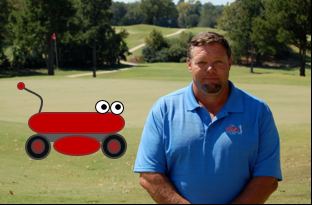
\includegraphics[width=6cm, valign=t]{usecase1_1.png} & 
Meet Steve. He's a golf course superintendent responsible for keeping the golf course looking professional. To save his groundskeeping team time, Steve just bought a GroundsBot unit to autonomously mow the rough around his golf course. \\
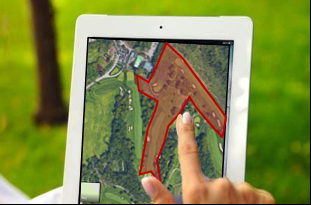
\includegraphics[width=6cm, valign=t]{usecase1_2.png} &
To start the mowing process, Steve first has to draw an outline of the area he wants mowed. He also highlights any zones Groundsbot should avoid while mowing.
\\
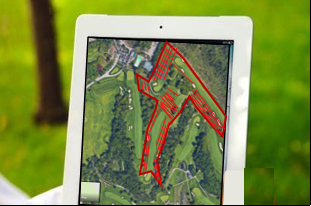
\includegraphics[width=6cm, valign=t]{usecase1_3.png} &
With the area to mow now outlined, the Groundsbot planning software creates a global route to cover the requested area. It avoids large obstacles like fairways, forests, and parking lots.
\\
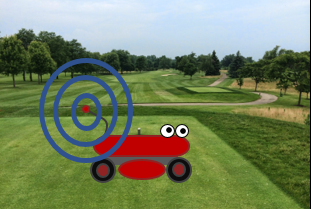
\includegraphics[width=6cm, valign=t]{usecase1_4.png} &
GroundsBot recieves the global route and localizes through GPS to determine where it is on the golf course.
\\
\end{tabularx}
\end{table}

\begin{table}[H]
   \def\arraystretch{4}
   \setlength\tabcolsep{8pt}


\begin{tabularx}{\textwidth}{cX}
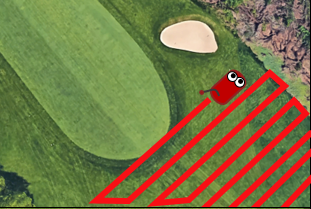
\includegraphics[width=6cm, valign=t]{usecase1_5.png} &
With the unit located and a global plan uploaded, GroundsBot begins mowing the area specified by Steve. It moves back and forth cutting the grass precisely, matching the quality care provided by Steve and his groundskeeping team.
\\
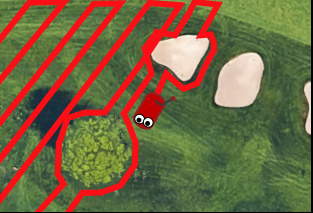
\includegraphics[width=6cm, valign=t]{usecase1_6.png} &
If GroundsBot encounters unplanned obstacles like sand bunkers or trees, GroundsBot avoids the obstacle and cuts around it. Once GroundsBot has avoided the obstacle in its path, it continues with the original plan.
\\
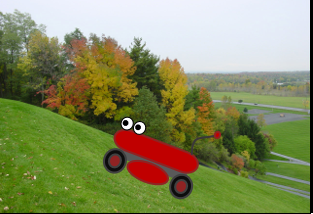
\includegraphics[width=6cm, valign=t]{usecase1_7.png} &
In order to maximize coverage, GroundsBot will navigate difficult terrain on a golf course, cutting the rough on steep hills.
\\
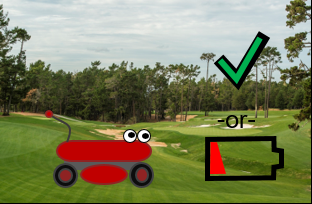
\includegraphics[width=6cm, valign=t]{usecase2_1.png} &
Once GroundsBot is finished or low on power, it notifies Steve and returns back home to be charged.
\\

\end{tabularx}
\end{table}

\begin{table}[H]
   \def\arraystretch{4}
   \setlength\tabcolsep{8pt}


\begin{tabularx}{\textwidth}{cX}
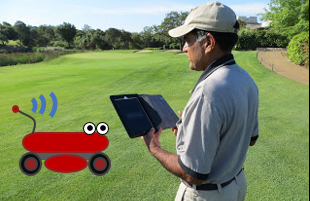
\includegraphics[width=6cm, valign=t]{usecase2_2.png} &
GroundsBot collected a lot of data while it was out cutting. It transfers diagnostics, coverage reports, and cutting data to Steve’s mobile device.
\\
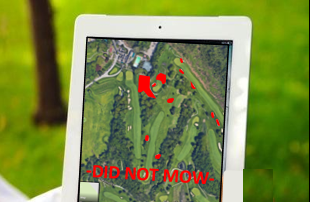
\includegraphics[width=6cm, valign=t]{usecase2_3.png} &
From here, Steve can analyze what areas of the course GroundsBot missed and what areas he has to send his team out to trim or tidy up.
\\
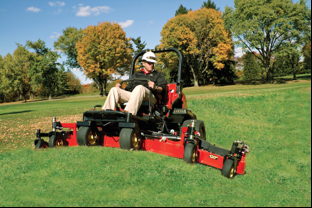
\includegraphics[width=6cm, valign=t]{usecase2_4.png} &
Steve sends out his groundskeeping team to quickly address missed spots or edging. This is a much faster experience for the team because they only have to touch up a few areas on the course.
\\
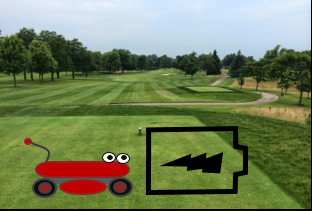
\includegraphics[width=6cm, valign=t]{usecase2_5.png} &
With the course looking professional, Steve and his groundskeeping team are happy they don’t have to worry about mowing the rough. GroundsBot recharges to prepare for another day of mowing.
\\

\end{tabularx}
\end{table}


\newpage
\section{System Level Requirements}

The system requirements were decided upon to demonstrate a proof of concept autonomous lawn mower that can be set up with minimal added infrastructure. To accomplish this, GroundsBot shall accept mowing regions from a user, cut the rough at the desired quality, and avoid any obstacles along the way.

\subsection{Mandatory Requirements}
\begin{center}
  \begin{table}[H]
  \caption{Mandatory Performance Requirements}
  \label{table:mandatory performance}

  \def\arraystretch{1.5}
  	\begin{tabularx}{\textwidth}{ lXX }
  	  \hline

		\sffamily\normalsize{ID} & \sffamily\normalsize{Requirement} & \sffamily\normalsize{Description} \\

    M.P.1 & First time user inputs map within 15 minutes & GroundsBot should be easy to use\\

    M.P.2 & System returns proposed route/coverage map within 5 minutes & Related to M.P.1 GroundsBot should start up quickly to ease the mind of the user\\

    M.P.3 & Cover 1/8 acre in 30 minutes on flat and unobstructed terrain & Minimum performance in ideal conditions\\

    M.P.4 & Cut 0-25\% overlap for 95\% of grass &  GroundsBot maintains an overlap with previous cut of no less than 0\% and no more than 25\% for 95\% of covered area.\\
    M.P.5 & Navigate 30 degree sloped grass & GroundsBot should be able to handle steep slopes safely\\

    M.P.6 & Detect 80\% of static objects greater than 3 inches in height and 2 inches in width & GroundsBot should be able to recognize static obstacles in order to prevent collisions and mowing accidents\\

    M.P.7 & Detect 80\% of dynamic objects greater than 6 inches in height and 6 inches in width travelling less than 4 mph &  GroundsBot should be able to recognize obstacles in order to prevent collisions and mowing accidents\\

    M.P.8 & Mow to within 1 foot of detected obstacles &  GroundsBot should be able to detect an obstacle (M.P.6) and navigate around it to continue its mowing path\\

    M.P.9 & Return home to within 5 feet of starting position & GroundsBot should return to its starting position to remove as much hassle from the user as possible\\
    
	\end{tabularx}
  \end{table}
\end{center}

\subsection{Desirable Performance Requirements}
\begin{center}
  \begin{table}[H]
  \caption{Desirable Performance Requirements}
  \label{table: desirable performance}
  

  \def\arraystretch{1.5}
  \begin{tabularx}{\textwidth}{ lXX }
      \hline
	  \sffamily\normalsize{ID} & \sffamily\normalsize{Requirement} & \sffamily\normalsize{Description} \\
	  D.P.1 & Mow to within 3 inches of a detected obstacles & A stretch goal for when M.P.8 (mow within 1 ft. of obstacles) is achieved\\

D.P.2 & Visually report mowing coverage and obstacles encountered & GroundsBot should report areas it missed to the user so the user knows where to manually mow to achieve full coverage\\

D.P.3 & Deck adjustable 0.5” to 2” & GroundsBot should be able to meet the grass height standards of different golf courses\\
  \end{tabularx}
  \end{table}
\end{center}

\subsection{Mandatory Non-Functional Requirements}
\begin{center}
  \begin{table}[H]
   \caption{Mandatory Non-Functional Requirements}
    \label{table: mandatory non-functional}
    

    \def\arraystretch{1.5}
    \begin{tabularx}{\textwidth}{ lXX }
     \hline
  	 \sffamily\normalsize{ID} & \sffamily\normalsize{Requirement} & \sffamily\normalsize{Description} \\  
  	  M.N.1 &
  	  Have a functional and easily accessible emergency stop &
  	  GroundsBot should be safe to use and easy to shut down in case of emergency\\
  	  M.N.2 &
  	  Be clearly visible &
  	  GroundsBot should indicate its presence and status to everyone nearby \\
  	  M.N.3 &
  	  Do not tear up grass &
  	  GroundsBot should not ruin any area it travels over \\
  	\end{tabularx}
  \end{table}
\end{center}

\subsection{Desirable Non-Functional Requirements}
\begin{center}
  \begin{table}[H]
  	\caption{Desirable Non-Functional Requirements}
  	\label{table: desirable non-functional}

  	\def\arraystretch{1.5}
	\begin{tabularx}{\textwidth}{ lXX }
  	\hline
  	  \sffamily\normalsize{ID} & \sffamily\normalsize{Requirement} &
  	  \sffamily\normalsize{Description} \\
  	  D.N.1 &
  	  Operates in variable lighting conditions &
  	  GroundsBot should operate at night to avoid interrupting golfers\\
	\end{tabularx}
  \end{table}
\end{center}


\newpage
\section{Functional Architecture}
  GroundsBot has to perform several key activities in order to produce mowed grass from a given mowing region.  GroundsBot must receive the intended mowing region from the user.  It must use these mowing regions to generate a mowing plan.  From here, the system starts its main mowing loop where it localizes itself, identifies obstacles to generate a map the navigate with.  GroundsBot uses this map and the mowing plan to plan a trajectory to avoid obstacles and maximize coverage.  This trajectory is converted to motor commands that are used to move the platform in the right direction to mow grass.  The end result is the mowing regions' grass is cut and the system can continue on to mowing more regions\\
  
\begin{figure}[H]
\centering
\def\svgwidth{\columnwidth}
\includegraphics[width=17cm, valign=t]{img/functionalArchitecture.jpg}
\caption{Functional Architecture}
\label{fig:functional}
\end{figure}

\newpage
\section{Cyberphysical Architecture}
The cyberphysical architecture is shown in Figure \ref{fig:cyberphysical}.  The user interacts with the GroundsBot system through a user-interface that allows them to use a satellite map to select mowing regions.  The user-interface connects and uploads the mowing regions to the GroundsBot platform via Wi-Fi.  The GroundsBot platform receives the intended mowing region and generates a mowing plan using a coverage planning algorithm.

GroundsBot uses an RTK GPS\cite{swiftnav} along with IMU and wheel odometry data to determine its position.  To identify obstacles, GroundsBot uses a stereo-camera and surface identification algorithms to build a map of the environment.  Using the map and the mowing plan, GroundsBot plans a trajectory to mow the grass using a local motion planning algorithm.  The trajectory is converted to motor velocities which are sent to the microcontroller that controls the motor controller.  The microcontroller sends an RC signal to the motor controller to drive the motors.  The motors drive the platform and mowing apparatus forward; mowing the grass and covering the mowing region.
\begin{figure}[H]
\centering
\def\svgwidth{\columnwidth}
\includegraphics[width=17cm, valign=t]{img/cyberPhysicalArchitecture.jpg}
\caption{Cyberphysical Architecture}
\label{fig:cyberphysical}
\end{figure}
  

\newpage
\section{Current System Status}
  \subsection{FVE Targeted System Requirements}
  It was decided to use the FVE to show progress towards meeting many of the system requirements rather than test for the requirements explicitly. Progress demonstrated on various system requirements is described in Table 5.
  
  \begin{center}
  \begin{table}[H]
  \caption{Targeted System Requirements}
  \label{table:targeted requirements}

  \def\arraystretch{1.5}
  	\begin{tabularx}{\textwidth}{ lXX }
  	  \hline

		\sffamily\normalsize{ID} & \sffamily\normalsize{Requirement} & \sffamily\normalsize{Target} \\

    M.P.1 & First time user inputs map within 15 minutes & Progress demonstrated with the Google Earth UI being used to generate waypoints.\\

    M.P.3 & Cover 1/8 acre in 30 minutes on flat and unobstructed terrain & Progress demonstrated with the platform demo. GroundsBot was shown to be able to navigate quickly and autonomously.\\

    M.P.4 & Cut 0-25\% overlap for 95\% of grass &  Progress demonstrated with the platform demo and grass classifcation demo. Groundsbot can navigate with high repeatability and can correctly classify grass cut to different heights.\\
    
    M.P.5 & Navigate 30 degree sloped grass & Progress demonstrated with the plaform demo. GroundsBot can safely climb and traverse moderately sloped hills.\\

    M.P.6 & Detect 80\% of static objects greater than 3 inches in height and 2 inches in width & Progress demonstrated with the classification demo. GroundsBot can detect things that are not grass.\\

    M.P.9 & Return home to within 5 feet of starting position & Progress demonstrated with the platform demo. GroundsBot returned to it's starting point at the end of the demonstration.\\
    
    M.N.1 & Have a functional and easily accessible emergency stop & Progress demonstrated with safety demo. GroundsBot has a safety tether which, when pulled, will quickly brake GroundsBots motors. \\
    
    M.N.3 & Do not tear up grass & Progress demonstrated with platform demo. Groundsbot was able to traverse a field without ruing the grass. \\
    
	\end{tabularx}
  \end{table}
\end{center}
  
  \subsection{Subsystem Status}
   	\subsubsection{UI}
  	It is critical for the user to communicate a desired mowing path to the robot. This input method must be separate from the robot itself, allowing the user to be somewhere else as the robot mows autonomously. 
  
  	This will be achieved through a mobile device, either a dedicated tablet or the user's own smartphone. An app or website will be loaded onto this device and allow for the user to input a map outline of the rough which will be converted to a target mowing region that is sent to the robot.
  
 	\subsubsection{Mowing Platform}
  		The mowing platform consists of a differential drive vehicle that carries an off-the-shelf mower. The frame of the vehicle is made mostly from aluminum extrusions. Two motors provided by Discovery Robotics are held on with a custom made aluminum mounting block. \colorbox{pink}{10 inch wheels are used in the rear, with a 5 inch caster in the front.} The off-the-shelf mower used was a Worx WG770 cordless electric mower, whose mowing deck was removed and then attached to the carrier vehicle.
    
  	  The entire system is powered off of the original Worx mower battery. The 36v battery was rewired to provide both a 36v and a 24v output. The 36v output powers the motor blade motor, while the 24v output powers the  motors as well as the other electronics.
    
  	  A custom PCBA was made to interface the sensors with an Arduino Mega, which serves as the bridge between the Nvidia Jetson TX2 and the Roboclaw motor controllers. The Arduino listens for messages coming in from either an RC transmitter or the Jetson, converts the message into a PWM output, and then passes this output along to the motor controller, which then provides the correct voltages to the motors. 
   
		With regards to safety, a tether was installed on the robot to short the motor connections when pulled, resulting in the motors braking. The motors are connected to their power source via relays which shut off when an undervoltage is detected, preventing damage to the battery. Fuses are also used throughout the platform to protect components from current surges. 
      

	 \subsubsection{Navigation}
 
      The navigation subsystem will develop a coverage plan based on the mowing region input that was received, localize the robot using data from its sensors, and then move the robot in a way that will follow the coverage plan. 
      
      Data from an IMU, an RTK GPS, as well as motor odometry will be fused together through a dual Extended Kalman Filter to provide information on where the robot is. Based on the robot's current location, the navigation subsystem will calculate the motor velocities needed to move the robot towards the next goal in its plan.
      
	\subsubsection{Perception \& Mapping}
    
    The perception \& mapping subsystem is responsible for using stereo image data to both detect obstacles as well as refine the map boundary that is received from the UI.  
    
    Obstacle detection will be done with object detection through both the stereo image depth information as well as the image pixel values. The images will be gathered from a Bumblebee XB3 stereo camera that is connected to the Jetson via Firewire. 
      
    A online grass classification algorithm will be used to refine the boundary inputs. This algorithm consists of two states, a learning state and a classification state. When the GPS sensor indicates that the robot is far from inputted boundary, the algorithm will go into its learning state, updating the model based on whether the robot is deep into either the fairway or the rough. When it approaches a boundary, the algorithm will switch into its classification state. The moment when output of algorithm in this state switches from fairway to rough or vice versa, the boundary stored in the map will be updated.  
  \subsection{Modeling, Analysis and Testing}
  
  \subsection{FVE Performance}
  GroundsBot performed as anticipated for the FVE and FVE encore.  The demonstrations consisted of three tests showing progress towards meeting system requirements.
  \subsubsection{Test 1: Waypoint Following}
  Test 1 demonstrated GroundsBot's ability to localize and navigate using GPS RTK. 5 waypoints were established prior to the test and marked with yellow cones. GroundsBot was tasked with navigating to each cone with a 2 foot tolerance, which was accomplished handily. Due to the time constraints of the FVE demo, long term repeatability was difficult to demonstrate, so the test procedure was later replicated for 6 trials. The mean distance to waypoints was measured at 6 inches with a standard deviation of 3.5 inches. 
  \subsubsection{Test 2: Grass Classification}
  Test 2 demonstrated the ability to classify grass types by training a classifier at run time. This can be used for correcting user defined mowing boundaries (rough vs. fairway vs. greens). For FVE, the classifier was trained at the Bob O'Connor Golf Course and test images were captured. The classifier classified the images live at the FVE on a laptop with an accuracy of 98\%, exceeding the requirement of 90%.
    
  The team felt the post processing during the demonstration failed to convey how the system is intended to work. For the FVE encore, a video was generated at Bob O'Connor Golf Course depicting the training and classification stages with an overlay showing accuracy (with ground truth provided by a GroundsBot team member in real time). The classifier distinguished rough and fairway grasses with an accuracy of 91.8\%.
  \subsubsection{Test 3: Emergency Stop}
  The third test demonstrated GroundsBot's emergency stop capability. The specification was to come to a halt within 2 seconds of a safety tether being pulled. GroundsBot stopped in well under 1 second. In addition to the specified test, a remote control emergency stop was also demonstrated.
  
  \subsection{System Status Conclusion}
  Overall, GroundsBot performed well on all demonstrations. In particular, the GroundsBot platform has proven to be very robust, has consistently navigated to waypoints accurately, and has demonstrated several layers of safety.

At present, weaknesses of the system are inability to navigate to waypoints within 1 meter of each other, inability to demonstrate long term GPS stability, and occasional ring terminal failures on motor connections. The navigation issue will be readily resolved in the spring with planned improvements to local planning algorithm. A fixed mount for the RTK base station will be deployed near the Doherty apartments test site such that long term GPS accuracy can be demonstrated. Finally, more robust ring terminals will be installed to prevent future failures.

\section{Project Management}
\subsection{Work Plan}
Figure \ref{fig:wbs} shows the GroundsBot work breakdown structure, a hierarchical encapsulation of deliverables critical to meeting system requirements. Items highlighted in green are complete. Items highlighted in yellow are in progress. Items highlighted in red are yet to be started.
  
  Completed items were determined to be critical for FVE, and were consequently prioritized in the fall. The remaining deliverables will enable a successful SVE.
\begin{figure}[H]
\centering
\def\svgwidth{\columnwidth}
\includegraphics[width=13cm]{wbs}
\caption{Work Breakdown Structure}
\label{fig:wbs}
\end{figure}

  
\subsection{Schedule}
Figure \ref{fig:springschedule} depicts the GroundsBot schedule for spring 2018. Critical milestones include improved ROS simulation using camera data, completion of global and local planners, static and dynamic obstacle detection, and user interface app integration.  
	After a long push at the end of the fall semester, all subsystems required for FVE were completed, which keeps the team on schedule for the spring.

\begin{figure}[H]
\centering
\includegraphics[width=13cm]{spring_schedule}
\caption{Spring Schedule}
\label{fig:springschedule}
\end{figure}

\subsubsection{deleteme}

The full list of milestones is laid out below in Table \ref{Tab:table_milestones}\\ 

\begin{table}[H]
\def\arraystretch{1}

\caption{Project Milestones}
\label{Tab:table_milestones}


\begin{tabular}{ll}
\hline
\normalsize\sffamily{Deadline} & \normalsize\sffamily{Milestone}                            \\
\\
Progress Review 1 [OCT 17 2017] & Mechanical CAD Complete \\
    &Electrical CAD Complete                     \\
    &BOM Complete                                \\
    &Parts Ordered                               \\
    &ROS Environment Initialized                 \\
                                               \\
Progress Review 2 [OCT 26 2017] & Chassis Assembled with Mowing Apparatus     \\
    &ROS Simulation Environment Complete         \\
    &GPS RTK Base Station Complete               \\
                                              \\ 
Progress Review 3 [NOV 7 2017] 
    &GroundsBot System Integration Complete      \\
    &GPS RTK Integration Complete                \\
    &Control Systems Demo Complete               \\
                                              \\
Progress Review 4 [NOV 21 2017] 
  
    &GroundsBot Accepts GPS Waypoints            \\
    &GroundsBot Follows GPS Waypoints            \\
    &Teleoperation Test Complete                 \\
                                               \\
Fall Validation Experiment [NOV 28 2017] 
 
    &GroundsBot Follows Route From Web App       \\
    &GroundsBot Differentiates Grass From Other Objects \\
                                            \\
                                            
January 2018

    &Global Planning Algorithm Complete          \\
    &Static and Dynamic Obstacle Detection Complete\\
                                               \\
February 2018
  
    &Read User Map Input                        \\
    &GroundsBot Reroutes Around Obstacles       \\
                                              \\
March 2018 
  
    &Full Mapping UI Complete                   \\
    &GroundsBot Autonomously Cuts Lot           \\
                                              \\
April 2018 

    &Final System Tests Complete                \\                                            \\
\end{tabular}

\end{table}

\subsubsection{Progress Reviews}
\noindent
\textbf{Progress Review 1}: The goal for Progress Review 1 is to have all hardware design complete with parts on order. \\
 \textbf{Progress Review 2}: The goal for Progress Review 2 is to have an assembled frame/chassis, a full ROS simulation environment, and a completed GPS + RTK base station.\\

\subsection{System Validation Experiments}
\subsubsection{Fall Validation Experiment}

	The aim of the fall validation experiment is to test individual subsystems. As such many of the systems requirements set for GroundsBot will not be fully met. All tests to be performed have been designed to indicate significant progress towards reaching the system requirements. More specifically the team plans to test the base functionality of the mobility, localization, planning, and perception subsystems of GroundsBot. The details of the test are laid out below.
\\
\begin{center}
\textbf{Test 1:}
\end{center}
 \textbf{Location:} Field by Doherty Apartments \cite{interview-guenther}
\\
\textbf{Equipment:} GroundsBot, GroundsBot dock/RTK base station, laptop
\begin{enumerate}
  \item Power on GroundsBot next to its docking station
  \item Establish connection between GroundsBot and mobile device
  \item Input GPS waypoints following a typical zigzag pattern a groundskeeper might make when mowing a lawn
  \item Send waypoints to GroundsBot
  \item GroundsBot will navigate to each waypoint entered, in the order they were entered
  \item Once the last waypoint is reached, GroundsBot will navigate back to the docking station (Note: the docking station will not be one of the entered waypoints)
\end{enumerate}

\begin{center}
\textbf{Test 2:}
\end{center}
Test 2 has been designed to demonstrate base functionality of the perception subsystem. The team will present a perception algorithm capable of differentiating between grass (i.e. a mowable surface) and non-grass (i.e. a non-mowable surface.) This test will be performed outside of the fall validation experiment and a replay of the test will be displayed during the fall validation experiment.

\newpage
\subsubsection{Spring Validation Experiment}

	The spring validation experiment will be when the team will test the full GroundsBot system to demonstrate that all system requirements have been met. The details of the test are laid out below.

\begin{center}
 \textbf{Test 1: }
\end{center}
\textbf{Location:} Field by Doherty Apartments\\
\textbf{Equipment:} GroundsBot, GroundsBot RTK base station, laptop, Five obstacles (one at minimum of performance requirements)\\
\textbf{Procedure:}
\begin{enumerate}
\item Power on GroundsBot

\item Open UI on laptop and establish a connection with GroundsBot

\item  Have a new user use UI to define boundaries of area to be mowed

\item  Use the UI to submit the mowing area to GroundsBot

\item  Area shall contain 5 static obstacles, such as trees, bushes, boxes etc..., one of which is minimum size from performance requirements

\item  GroundsBot will develop a coverage plan of the area input by the user

\item  GroundsBot mows area per performance requirements

\item  GroundsBot returns to starting position per performance requirements
\end{enumerate}

\noindent
\textbf{Criteria:}

\begin{enumerate}
\item M.P.1: First time user inputs map within 15 minutes
\item M.P.2: System returns proposed route within 5 minutes
\item M.P.3: Cover 1/8 acre in 30 minutes
\item M.P.4: Cut 0-25\% overlap for 95\% of grass
\item M.P.6: Detect 80\% of static objects > 3"x2"x2"
\item M.P.8: Mow within 1' of detected obstacles
\item M.P.9: Return home to within 5' of starting position
\end{enumerate}

\begin{center}
 \textbf{Test 2: }
\end{center}
\textbf{Location:} Field by Doherty Apartments\\
\textbf{Equipment:} GroundsBot, GroundsBot RTK base station, laptop, soccer ball\\
\textbf{Procedure:}
\begin{enumerate}
\item GroundsBot is directed to move in a straight line

\item Team throws a soccer ball in front of GroundsBot 5 times

\item GroundsBot stops until obstacle is out of range per performance requirements
\end{enumerate}

\noindent
\textbf{Criteria:}
\begin{enumerate}
\item M.P.7: M.P.7: Detect and avoid 80\% of dynamic objects greater than 6”x6”x6” travelling less than 4 mph

\end{enumerate}

\begin{center}
 \textbf{Test 3: }
\end{center}
\textbf{Location:} Test conducted offline\\
\textbf{Equipment:} GroundsBot\\
\textbf{Procedure:}
\begin{enumerate}
\item Power on GroundsBot
\item Manually control GroundsBot up 30 degree hill with RC transmitter
\end{enumerate}

\noindent
\textbf{Criteria:}

\begin{enumerate}
\item M.P.5: Navigate 30 degree sloped grass
\end{enumerate}


\subsection{Budget}
The total budget for GroundsBot is \$5000, of which \$3959.22 (79\%) has been spent and \$1040.78 remains. The largest expenditures to date are the Emlid Reach GPS RTK Kit, the Nvidia Jetson TX2 cpu, the electric mower base, GPS antennas, spare 36V batteries, and motor drivers. A complete bill of materials is shown in Appendix A.

\begin{center}
\begin{table}[H]
\def\arraystretch{1}

\caption{Bill of Materials}
\label{Tab:bom}


\begin{tabular}{llll}
\hline
\normalsize\sffamily{Category} & \normalsize\sffamily{Details} & \normalsize\sffamily{Quantity} & \normalsize\sffamily{Cost}                            \\
Chassis & Misc Parts & 1 & \$854.28\\
GPS & Reach RTK Kit & 1 & \$570.00\\
CPU & Nvidia Jetson TX2 & 1 & \$300.00\\
Mowing & Worx Cordless Mower & 1 & \$289.33 \\
GPS & GNSS Antenna & 2 & \$390.00 \\
Battery & Spare 36V Battery & 2 & 279.98 \\
Electronics & Roboclaw Motor Driver & 2 & \$179.90 \\
\end{tabular}
\end{table}
\end{center}

\subsection{Risk Management}
\begin{table}[H]
\def\arraystretch{1.7}

\begin{tabular}{p{7cm}p{6cm}c}
 {Risk} &  {Management Strategy} &  {Risk Category}\\
\hline 
 \textbf{Too Few Features for Perception:} 
If we cannot consistently detect grass from non-grass features, perception subsystem will not be able to direct platform accurately
&
Install infrastructure such as fiducials to assist system in recognizing objects.
&
Technical\\

 \textbf{Team Falling Behind Due to Work:} 
Team may overestimate capability and overwhelm itself with assignments.
&
Prepare for risk by managing tasks and using buffer weeks. Mitigate effect by delaying milestones or cutting compromising targets.
&
Schedule\\
 \textbf{Localization Poor for Following Edges:} 
If our localization algorithms cannot accurately follow edge of lawn, system will not mow lawn effectively.
&
Prepare by understanding criticality of localization. Mitigate effect by changing scope of mowing problem or adding infrastructure to assist.
&
Technical\\
 \textbf{Injury from Spinning Blade:} 

Our system has a dangerous cutting instrument. It can injure a team member or a bystander.
&
Prepare by making sure team understands the risk of spinning blade. Put warning lights and sounds to alert bystanders when testing.
&
Technical\\

 \textbf{Poor Weather for Validation Experiments:} 
Poor weather on demonstration days would prevent us from system from performing.
&
Team monitors upcoming weather before validation experiments.  Records the validation experiment before hand and replays in the case of inclement weather conditions.
&
Schedule\\

 \textbf{Team Member Has Family Constraints:} 
Any team member could experience a family emergency or responsibility that occupies their time and focus. One specific concern is Josh's wife is pregnant and expecting in December.
&
Mitigate the effect on entire team by spreading work across several team members and communicating consistently with absent team member to keep them in the loop.
&
Personal\\

 \textbf{Platform Devastating Event:} 
Platform could have electrical, thermal, or kinetic event that leads to its destruction.
&
Team designs platform with risk in mind, and manages parts reserve to quickly rebuild platform if necessary.
&
Technical\\

 \textbf{Subsystem Harder Than Expected:} 
Any subsystem could require more work than expected, taking away focus from other subsystems.
&
Team can prepare by focusing on critical subsystems first, and may revise scope related to subsystem if necessary.
&
Technical\\

\textbf{Not Enough Capital for Development:} 
There is a risk our system requires more money than initially allocated.
&
To mitigate the effect of this event, team will maintain strong relationship with sponsor by providing consistent communication of development progress. Team may also reach out to other sponsors or donors.
&
Schedule\\
\end{tabular}
\end{table}

\section{Conclusions}
GroundsBot has come a long way, and so has the GroundsBot team. While GroundsBot learned to move, localize, and navigate, the team also learned some new things. First, we found pair programming to be an invaluable tool for debugging. Allocating multiple team members to a problem allowed for better distribution of knowledge and increased velocity on critical tasks. We will employ this tactic even more frequently in the spring. In retrospect, we also found that we failed to adhere to our project management workflow consistently. We consistently maintained good communication between team members, but a lot of decisions remained undocumented which hurt us long term. We aim to be more rigorous with our Asana board in the spring. Lastly, we learned the importance of making robots carry equipment for you. Lesser teams might carry equipment to a test site manually, but GroundsBot takes care of that for us. We aim to make full use of GroundsBot's towing capacity to accelerate future testing. And also to transport our snacks.

\begingroup
\newpage
\section{References}
\renewcommand{\section}[2]{}% %Suppress bibliography header, doesn't work with toc
\begin{thebibliography}{}
\bibitem{clubbenchmarking} 
http://www.clubbenchmarking.com/blog/golf-course-maintenance-how-much-should-you-spend
\bibitem{husky} 
https://www.clearpathrobotics.com/husky-unmanned-ground-vehicle-robot/
\bibitem{husqvarna} 
http://www.husqvarna.com/us/products/robotic-lawn-mowers/
\bibitem{swiftnav} 
https://www.swiftnav.com/store?category=GNSS+Modules
\bibitem{superdroid} 
https://www.superdroidrobots.com/shop/item.aspx/prebuilt-2wd-66in-lawn-mower-wc-sold/1983/
\bibitem{interview-duxbury} 
Duxbury, Jeff [Bob O’Connor Golf Course Superintendent]. (2017, September 16). Personal interview.
\bibitem{interview-guenther} 
Guenther, Steve [Carnegie Mellon University Director of Facilities Operations]. (2017, September 22). Personal interview.
\end{thebibliography}
\endgroup

\begin{appendices}
\chapter{Appendix A}

\begin{table}[H]
\centering
\def\arraystretch{1.1}
\caption{Bill of Materials}
\label{Tab:bom}
\begin{tabular}{ llccl }
\hline
    \normalsize\sffamily {Component} & \normalsize\sffamily {Quantity} & \normalsize\sffamily {Unit Cost} & \normalsize\sffamily {Total Cost} 
    \\[-.8ex]
Worx WG770 36V Cordless Mower	&	1	&	\$289.33	&	\$289.33	\\
REACH RTK KIT	&	1	&	\$570.00	&	\$570.00	\\
3DR 915 Mhz (US) Telemetry Radio	&	1	&	\$0.00	&	\$49.99	\\
Simple-H 20A, 5V to 28V DC Motor Driver	&	2	&	\$47.95	&	\$95.90	\\
DC/DC CONVERT	&	1	&	\$448.05	&	\$448.05	\\
8-Channel 2.4ghz Receiver	&	1	&	\$35.97	&	\$35.97	\\
1/4"-20 Thread Swivel Security Camera Mount	&	1	&	\$8.89	&	\$8.89	\\
Gray Rubber Wheel	&	1	&	\$43.18	&	\$43.18	\\
Robot Drive Wheel - 10 inch Pneumatic	&	2	&	\$7.90	&	\$15.80	\\
Flange-Mount Shaft Collar, 20 mm diameter	&	2	&	\$63.58	&	\$127.16	\\
18-8 Stainless Steel M6 16mm Screw	&	1	&	\$7.28	&	\$7.28	\\
6mm Key Stock, Stainless Steel	&	1	&	\$9.22	&	\$9.22	\\
6061 Sheet, 3/8" thick, 5"x24"	&	1	&	\$31.35	&	\$31.35	\\
6061 Sheet, 1/8" thick, 18"x18"	&	1	&	\$59.98	&	\$59.98	\\
6061 Sheet, 1/8" thick, 6"x6"	&	1	&	\$9.60	&	\$9.60	\\
Panduit Slotted Duct, 0.5" x 1" White, 6 Feet	&	6	&	\$3.92	&	\$23.52	\\
Panduit Duct Cover, 0.5" White, 6 Feet	&	6	&	\$1.03	&	\$6.18	\\
Anchor Connector for 1" High Rail	&	36	&	\$3.39	&	\$122.04	\\
Handle for 1" Rail Height	&	4	&	\$6.40	&	\$25.60	\\
4 FT OPTION, Double Rail, Silver, 2" High x 1" Wide, Solid	&	3	&	\$22.98	&	\$68.94	\\
80/20 1"x1" Quarter Round Extrusion	&	1	&	\$6.75	&	\$6.75	\\
80/20 1"x0.5" Extrusion	&	1	&	\$13.47	&	\$13.47	\\
Spring-Loaded Ball Fastener for 1" High Rail	&	60	&	\$1.12	&	\$67.20	\\
Stainless Steel Screw, 10-32 Thread 1/2" Long	&	1	&	\$6.11	&	\$6.11	\\
Anchor Connector for 1" High Rail	&	2	&	\$3.39	&	\$6.78	\\
Omron Industrial Relay	&	2	&	\$46.90	&	\$93.80	\\
Pack of 50 Single-level Screwless Terminal Block	&	1	&	\$24.00	&	\$24.00	\\
Fuse Terminal Block	&	1	&	\$20.00	&	\$20.00	\\
Relay Bracket	&	2	&	\$1.08	&	\$2.16	\\
Circuit Breaker	&	1	&	\$18.50	&	\$18.50	\\
Pack of 25A Fuses	&	1	&	\$7.25	&	\$7.25	\\
Pack of 15A Fuses	&	1	&	\$4.75	&	\$4.75	\\
Pack of 10A Fuses	&	1	&	\$4.75	&	\$4.75	\\
Terminal Block End Cover	&	1	&	\$12.00	&	\$12.00	\\
Terminal Block Jumper	&	1	&	\$17.00	&	\$17.00	\\
DIN Rail	&	1	&	\$9.00	&	\$9.00	\\
Pluggable Terminal Block	&	1	&	\$1.35	&	\$1.35	\\
White Pluggable Terminal Block	&	1	&	\$0.74	&	\$0.74	\\
Pre-Crimped Wire Leads	&	80	&	\$0.35	&	\$27.92	\\
Receptacle Housing 6 Position Microfit	&	10	&	\$0.36	&	\$3.56	\\
Receptacle Housing 4 Position Microfit	&	10	&	\$0.30	&	\$3.00	\\
Receptacle Housing 2 Position Microfit	&	10	&	\$0.23	&	\$2.34	\\
Button Head Screw 3/8-16 Thread	&	1	&	\$5.03	&	\$5.03	\\
Button Head Screw 8-32 Thread	&	1	&	\$3.71	&	\$3.71	\\
Button Head Screw 4-40 Thread	&	1	&	\$2.71	&	\$2.71	\\
Threaded 4-40 Standoff 0.5 in Length	&	12	&	\$1.87	&	\$22.44	\\
Threaded 4-40 Standoff 1.5 in Length	&	4	&	\$2.39	&	\$9.56	\\
Threaded 4-40 Standoff 1.0 in Length	&	2	&	\$2.22	&	\$4.44	\\
Threaded 4-40 Standoff 3/16 in Length	&	2	&	\$2.59	&	\$5.18	\\
Kill Switch	&	1	&	\$15.94	&	\$15.94	\\
\end{tabular}
\end{table}

\begin{table}[H]
\centering
\def\arraystretch{1.1}
\caption{Bill of Materials page 2}
\label{Tab:bom2}
\begin{tabular}{ llccl }
\hline
    \normalsize\sffamily {Component} & \normalsize\sffamily {Quantity} & \normalsize\sffamily {Unit Cost} & \normalsize\sffamily {Total Cost} 
    \\[-.8ex]

M6 Avikrimp ring terminal	&	10	&	\$0.43	&	\$4.30	\\
1394a PCI Express FireWire Card Adapter	&	1	&	\$28.30	&	\$28.30	\\
M6 Avikrimp ring terminal	&	15	&	\$0.65	&	\$9.75	\\
RoboClaw 2x15A Regenerative Motor Controller	&	1	&	\$89.95	&	\$89.95	\\
Pluggable Terminal Block 3 Pos	&	3	&	\$8.43	&	\$25.29	\\
Pluggable Terminal Block 3 Pos Connector	&	2	&	\$5.33	&	\$10.66	\\
Lead Acid 24V 2.0A Charger	&	1	&	\$16.99	&	\$16.99	\\
Kill Switch Normally Closed	&	1	&	\$19.43	&	\$19.43	\\
Relay Bracket	&	1	&	\$1.08	&	\$1.08	\\
Omron Industrial Relay	&	1	&	\$46.90	&	\$46.90	\\
CONN HEADER 6 POS 2.54	&	4	&	\$0.33	&	\$1.32	\\
Led, Green, 1.25mm x 1.4mm, 7mcd, 570nm, Full Reel	&	25	&	\$0.36	&	\$9.10	\\
RES SMD 60.4 OHM 1\% 1/10W 0603	&	25	&	\$0.15	&	\$3.75	\\
RES SMD 10K OHM 1\% 1/10W 0603	&	25	&	\$0.15	&	\$3.75	\\
CONN HEADER 30POS SMT VERT 30AU	&	2	&	\$4.79	&	\$9.58	\\
Smt t/r	&	4	&	\$1.22	&	\$4.88	\\
CONN HEADER 2POS RT ANG SMD TIN	&	16	&	\$2.57	&	\$41.12	\\
CONN HEADER 6POS RT ANG SMD TIN	&	10	&	\$3.21	&	\$32.10	\\
CONN HEADER 4POS RT ANG SMD TIN	&	8	&	\$2.89	&	\$23.12	\\
CAP CER 1UF 25V X5R 0603	&	10	&	\$0.06	&	\$0.60	\\
CAP CER 10UF 25V X5R 0603	&	10	&	\$0.29	&	\$2.85	\\
Fuse Chip Very Fast Acting 4A SMD	&	5	&	\$2.55	&	\$12.75	\\
VARISTOR 12V 60A 0805	&	2	&	\$0.49	&	\$0.98	\\
VARISTOR 5V 40A 0805	&	2	&	\$0.57	&	\$1.14	\\
RES SMD 470 OHM 1\% 1/10W 0603	&	10	&	\$0.10	&	\$1.00	\\
RES SMD 147 OHM 1\% 1/10W 0603	&	10	&	\$0.10	&	\$1.00	\\
RES SMD 2K OHM 5\% 1/10W 0603	&	25	&	\$0.10	&	\$2.50	\\
CONV DC/DC 2A 6.5-28VIN 5V	&	2	&	\$22.77	&	\$45.54	\\
MODULE DC/DC 1/16 BRICK 12V 4A	&	2	&	\$26.78	&	\$53.56	\\
NC7SZ04 Series 5.5 V SMT Logic UHS Inverter	&	2	&	\$0.38	&	\$0.76	\\
SCHOTTKY 60V 20A	&	2	&	\$1.48	&	\$2.96	\\
2x FUSE CLIP CARTRIDGE 600V 20A PCB	&	4	&	\$0.58	&	\$2.32	\\
RES SMD 47K OHM 1\% 1/10W 0603	&	25	&	\$0.10	&	\$2.50	\\
RES SMD 330K OHM 1\% 1/10W 0603	&	25	&	\$0.10	&	\$2.50	\\
IC OPAMP ISOLATION 100KHZ 8SOP	&	2	&	\$6.13	&	\$12.26	\\
Optocoupler DC-IN 1-CH Transistor 	&	2	&	\$1.06	&	\$2.12	\\
VARISTOR 33V 2KA DISC 20MM	&	2	&	\$0.95	&	\$1.90	\\
RES SMD 0 OHM JUMPER 1W 2512	&	10	&	\$0.18	&	\$1.80	\\
IC REG LINEAR 5V 50MA 8SOIC	&	2	&	\$2.04	&	\$4.08	\\
DIODE GEN PURP 75V 300MA SOD323	&	4	&	\$0.14	&	\$0.56	\\
RES SMD 52.3 OHM 1\% 1W 2512	&	10	&	\$0.39	&	\$3.90	\\
TRANS NPN 100V 3A SOT223	&	6	&	\$0.64	&	\$3.84	\\
RES SMD 750K OHM 1\% 1/10W 0603	&	10	&	\$0.10	&	\$1.00	\\
RES SMD 150K OHM 1\% 1/10W 0603	&	10	&	\$0.10	&	\$1.00	\\
RES SMD 180K OHM 1\% 1/10W 0603	&	10	&	\$0.10	&	\$1.00	\\
Low Voltage, Precision Comparator	&	2	&	\$2.00	&	\$4.00	\\
CONN TERM BLOCK 4POS 3.5MM	&	4	&	\$2.35	&	\$9.40	\\
CONN HEADER 6POS 1.25MM SMD GOLD	&	2	&	\$1.04	&	\$2.08	\\
4-Bit Bidirectional Multi-Voltage Level Translator	&	2	&	\$1.11	&	\$2.22	\\
9DoF IMU Breakout	&	2	&	\$24.95	&	\$49.90	\\
CBL RIBN 40COND 0.050 MULTI 5'	&	1	&	\$16.91	&	\$16.91	\\
CONN SOCKET 40 POS IDC W/STR REL	&	4	&	\$2.21	&	\$8.84	\\
Jumper Wire - 0.1", 6-pin, 12"	&	2	&	\$1.95	&	\$3.90	\\
DF13 6 Position Connector 30cm	&	1	&	\$6.55	&	\$6.55	\\
SparkFun 9DoF Sensor Stick	&	1	&	\$14.95	&	\$14.95	\\
BOX PLASTIC GRAY 7.09"L X 7.09"W	&	1	&	\$29.50	&	\$29.50	\\
Lead Acid 36V Battery	&	2	&	\$139.99	&	\$279.98	\\
Pluggable Terminal Block 3 Pos Connector	&	2	&	\$5.33	&	\$10.66	\\
Anchor Connector for 1" High Rail	&	25	&	\$3.39	&	\$84.75	\\
Battery Charger 12 V 2 Amps	&	1	&	\$20.88	&	\$20.88	\\
\end{tabular}
\end{table}

\begin{table}[H]
\centering
\def\arraystretch{1.1}
\caption{Bill of Materials page 3}
\label{Tab:bom3}
\begin{tabular}{ llccl }
\hline
    \normalsize\sffamily {Component} & \normalsize\sffamily {Quantity} & \normalsize\sffamily {Unit Cost} & \normalsize\sffamily {Total Cost} 
    \\[-.8ex]
GNSS Antenna Pack with Cables	&	2	&	\$195.00	&	\$390.00	\\
Socket Head Screw 5/8" Thread	&	1	&	\$2.97	&	\$2.97	\\
Lead Acid 24V 2.0A Charger	&	1	&	\$16.99	&	\$16.99	\\
Pluggable Terminal Block 3 Pos Connector	&	2	&	\$5.33	&	\$10.66	\\
Pluggable Terminal Block 3 Pos	&	2-1 Back ordered	&	\$8.43	&	\$16.86	\\
Battery Charger 12 V 2 Amps	&	1	&	\$20.88	&	\$20.88	\\
Ring Terminal Command	&	15	&	\$0.21	&	\$3.15	\\
RoboClaw 2x15A Regenerative Motor Controller	&	1	&	\$89.95	&	\$89.95	\\
TECHTOO® 9dBi Omni WiFi Antenna	&	1	&	\$10.99	&	\$10.99	\\
BumbleBee Stereo Camera	&	1	&	&	\\
Nvidia Jetson TX2 CPU & 1 & & 
\end{tabular}
\end{table}

\end{appendices}
\end{document}



\title{GroundsBot: Autonomous Golf Course Maintenance \\[.5ex]
		\Large Conceptual Design Review}
\date{September 2017}
\author{CMU MRSD Team A        \\ Sponsor: Discovery Robotics \\ David Evans \\
        Adam Driscoll \\ Henry Chen  \\
        Josh Bennett  \\ Joe Phaneuf \\ }

\maketitle
\def\svgwidth{\columnwidth}
\input{img/groundsbot_logo.pdf_tex}
\newpage

\begin{spacing}{0.95}
\tableofcontents
\end{spacing}

\newpage

\newpage
\section{Project Description}

People spend a lot of time mowing grass. This is particularly true for golf courses. Golf courses have hundreds of acres of land requiring careful maintenance. The median club in the United States spends \$1.2 million per year on maintenance \cite{clubbenchmarking}. A Pittsburgh area golf course superintendent \cite{interview-duxbury} revealed that his staff spends 65\% of their time mowing, and 60\% of that time is spent just on the rough. This is an industry ripe for automation.
\\

Autonomous mowers are commercially available today, however most of these units require buried wires, beacons, or extensive mapping to provide boundaries. For a golf course, the mowing area is so large that those setup methods are a barrier to deployment. The GroundsBot team aims to deliver an autonomous mower that can be deployed with minimal infrastructure, using a coarse boundary map provided by the user.

\newpage
\section{Use Case}
\begin{table}[H]
  \def\arraystretch{4}
   \setlength\tabcolsep{8pt}


\begin{tabularx}{\textwidth}{cX}
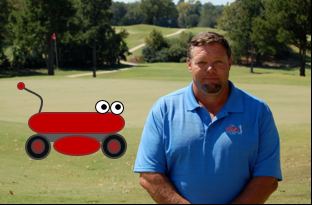
\includegraphics[width=6cm, valign=t]{usecase1_1.png} & 
Meet Steve. He's a golf course superintendent responsible for keeping the golf course looking professional. Right now, Steve and his groundskeeping team spend 65\% of their time just mowing grass. To save time, Steve just bought a GroundsBot unit to autonomously mow the rough around his golf course. \\
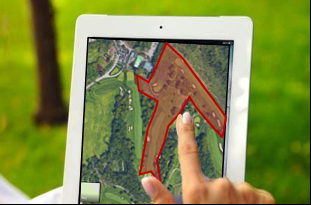
\includegraphics[width=6cm, valign=t]{usecase1_2.png} &
To start the mowing process, Steve first has to draw an outline of the area he wants mowed. He also highlights any zones Groundsbot should avoid while mowing.
\\
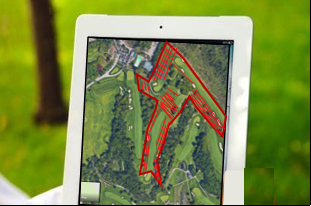
\includegraphics[width=6cm, valign=t]{usecase1_3.png} &
With the area to mow now outlined, the Groundsbot planning software creates a global route to cover all of the requested area. It avoids large obstacles like fairways, forests, and parking lots.
\\
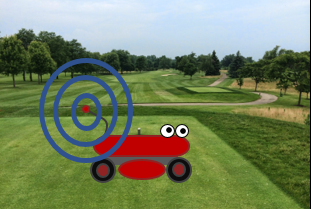
\includegraphics[width=6cm, valign=t]{usecase1_4.png} &
GroundsBot recieves the global route and localizes through GPS to determine where it is on the golf course.
\\
\end{tabularx}
\end{table}

\begin{table}[H]
   \def\arraystretch{4}
   \setlength\tabcolsep{8pt}


\begin{tabularx}{\textwidth}{cX}
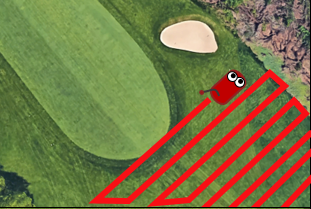
\includegraphics[width=6cm, valign=t]{usecase1_5.png} &
With the unit located and a global plan uploaded, GroundsBot begins mowing the area specified by Steve. It moves back and forth cutting the grass precisely, matching the quality care provided by Steve and his groundskeeping team.
\\
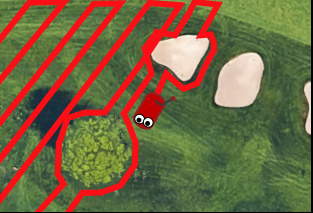
\includegraphics[width=6cm, valign=t]{usecase1_6.png} &
If GroundsBot encounters unplanned obstacles like sand traps or individual trees, GroundsBot avoids the obstacle and cuts around it. Once GroundsBot has avoided the obstacle in its path, it continues with the original plan.
\\
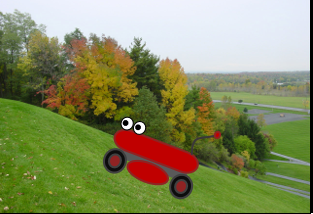
\includegraphics[width=6cm, valign=t]{usecase1_7.png} &
In order to maximize coverage, GroundsBot will navigate difficult terrain on a golf course, cutting the rough on steep hills.
\\
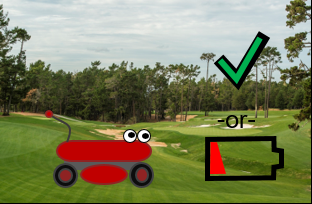
\includegraphics[width=6cm, valign=t]{usecase2_1.png} &
Once GroundsBot is finished or low on power, it notifies Steve and returns back to the charging dock.
\\

\end{tabularx}
\end{table}

\begin{table}[H]
   \def\arraystretch{4}
   \setlength\tabcolsep{8pt}


\begin{tabularx}{\textwidth}{cX}
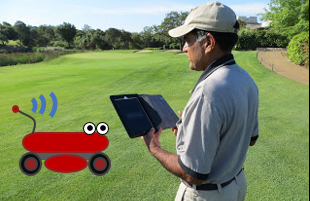
\includegraphics[width=6cm, valign=t]{usecase2_2.png} &
GroundsBot collected a lot of data while it was out cutting. It transfers diagnostics, coverage reports, and cutting data to Steve’s mobile device.
\\
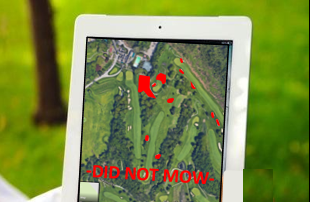
\includegraphics[width=6cm, valign=t]{usecase2_3.png} &
From here, Steve can analyze what areas of the course GroundsBot missed and what areas he has to send his team out to trim or tidy up.
\\
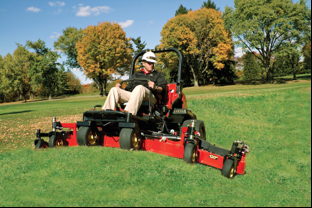
\includegraphics[width=6cm, valign=t]{usecase2_4.png} &
Steve sends out his groundskeeping team to quickly address missed spots or edging. This is a much faster experience for the team because they only have to touch up a few areas on the course.
\\
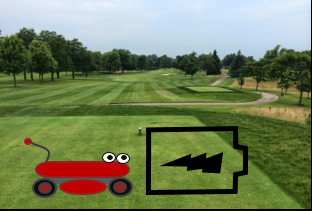
\includegraphics[width=6cm, valign=t]{usecase2_5.png} &
With the course looking professional, Steve and his groundskeeping team are happy they don’t have to worry about mowing. GroundsBot recharges to prepare for another day of mowing.
\\

\end{tabularx}
\end{table}


\newpage
\section{System Level Requirements}

The system requirements were decided upon to demonstrate a proof of concept autonomous lawn mower that can be set up with minimal added infrastructure. The only added infrastructure will be a docking station for GroundsBot. To accomplish this, GroundsBot must be able to localize with extreme accuracy in an unknown environment. GroundsBot must also be able to navigate consistently along a mowing path plan. Finally, GroundsBot must be able to detect and avoid any obstacles along the way.

\subsection{Mandatory Requirements}
\begin{center}
  \begin{table}[H]
  \caption{Mandatory Performance Requirements}
  \label{table:mandatory performance}

  \def\arraystretch{1.5}
  	\begin{tabularx}{\textwidth}{ lXX }
  	  \hline

		\sffamily\normalsize{ID} & \sffamily\normalsize{Requirement} & \sffamily\normalsize{Description} \\
    	M.P.1 &
    	First time user inputs map within 15 minutes &
    	GroundsBot should be easy to use \\
   		M.P.2 &
   		System returns proposed route/coverage map within 5 minutes &
   		Related to M.P.1, GroundsBot should start up quickly to ease the mind of the user \\
   		M.P.3 &
   		Cut 0-25\% overlap for 95\% of grass &
   		When mowing, GroundsBot should cut in a way that accomplishes full grass coverage while maintaining efficiency by reducing overlap\\
		M.P.4 &
		Mow 50$ft^2$ of 30 degree sloped grass &
		GroundsBot should be able to handle steep slopes to eliminate safety hazards \\
		M.P.5 &
		Detect 80\% of objects greater than 27 cubic inches &
		GroundsBot should be able to recognize obstacles in order to prevent collisions and mowing accidents \\
		M.P.6 &
		Mow to within 1 foot of detected obstacles &
		GroundsBot should be able to detect an obstacle (M.P.5) and navigate around it to continue its mowing path \\
		M.P.7 &
		Mow 90\% of a $\frac{1}{4}$ acre area &
		GroundsBot will encounter obstacles along the way preventing it from 100\% coverage \\
	\end{tabularx}
  \end{table}
\end{center}

\subsection{Desirable Performance Requirements}
\begin{center}
  \begin{table}[H]
  \caption{Desirable Performance Requirements}
  \label{table: desirable performance}
  

  \def\arraystretch{1.5}
  \begin{tabularx}{\textwidth}{ lXX }
      \hline
	  \sffamily\normalsize{ID} & \sffamily\normalsize{Requirement} & \sffamily\normalsize{Description} \\
	  D.P.1 &
	  Mow to within 3 inches of a detected obstacles &
	  A stretch goal for when M.P.6 (mow within 1 ft. of obstacles) is achieved \\
  	  D.P.2 &
  	  Visually report mowing coverage and obstacles encountered &
  	  GroundsBot should report areas it missed to the user so the user knows where to manually mow to achieve full coverage\\
  \end{tabularx}
  \end{table}
\end{center}

\subsection{Mandatory Non-Functional Requirements}
\begin{center}
  \begin{table}[H]
   \caption{Mandatory Non-Functional Requirements}
    \label{table: mandatory non-functional}
    

    \def\arraystretch{1.5}
    \begin{tabularx}{\textwidth}{ lXX }
     \hline
  	 \sffamily\normalsize{ID} & \sffamily\normalsize{Requirement} & \sffamily\normalsize{Description} \\
	  M.N.1 &
  	  Return home to within 5 feet of dock &
  	  GroundsBot should return to its starting position to remove as much hassle from the user as possible \\  	  
  	  M.N.2 &
  	  Have a functional and easily accessible emergency stop &
  	  GroundsBot should be safe to use and easy to shut down in case of emergency\\
  	  M.N.3 &
  	  Be clearly visible &
  	  GroundsBot should indicate its presence and status to everyone nearby \\
  	  M.N.4 &
  	  Do not tear up grass &
  	  GroundsBot should not ruin any area it travels over \\
  	\end{tabularx}
  \end{table}
\end{center}

\subsection{Desirable Non-Functional Requirements}
\begin{center}
  \begin{table}[H]
  	\caption{Desirable Non-Functional Requirements}
  	\label{table: desirable non-functional}

  	\def\arraystretch{1.5}
	\begin{tabularx}{\textwidth}{ lXX }
  	\hline
  	  \sffamily\normalsize{ID} & \sffamily\normalsize{Requirement} &
  	  \sffamily\normalsize{Description} \\
  	  D.N.1 &
  	  Operates in variable lighting conditions &
  	  GroundsBot should operate at night to avoid interrupting golfers\\
  	  D.N.2 &
  	  Deck adjustable 0.5” to 2” &
  	  GroundsBot should be able to meet the grass height standards of different golf courses\\
  	  D.N.3 &
  	  Bot is resistant to impacts &
  	  GroundsBot should be unaffected if hit by a golf ball while mowing\\
  	  D.N.4 &
  	  Return home to and mate with charging dock &
  	  A stretch goal if M.N.1 (return to within 5 ft. of dock) is achieved \\
	\end{tabularx}
  \end{table}
\end{center}


\newpage
\section{Functional Architecture}
  There are three subsystems that combine to accomplish the functionality needed for GroundsBot (Figure~\ref{fig:functional}). The User Interface accepts inputs from the groundskeeper, generating detailed mowing regions. The Charging Dock acts as a home point for charging the robot, while also providing a reference signal for correcting localization issues. The Mowing Robot includes internal subsystems which enable the robot to navigate the golf course, cut the rough, and return to the charging dock when needed.\\
  
\begin{figure}[H]
\centering
\def\svgwidth{\columnwidth}
\input{img/functional.pdf_tex}
\caption{Functional Architecture}
\label{fig:functional}
\end{figure}

\newpage
  The Mowing Robot subsystem is responsible for many critical tasks in the Autonomous Golf Rough Mowing system. The Vehicle Platform is one internal subsystem that ensures effective mowing operations by storing energy, providing mobility, and docking when charging is needed. The Mower Electronics subsystem provides electrical controls for the motors and hosts the computing resources needed to run the algorithms for mowing. The sensor data provided by this subsystem is crucial for the remaining systems, enabling full mowing autonomy.\\
  
  The remaining subsystems within the Mowing Robot include Online Perception, Robot Localization, Navigation Planning, and Control. These software systems provide GroundsBot with awareness of surroundings, knowledge of position, and in-depth details about the grass. This enables successful navigation through complicated environments, and provides the information necessary to control GroundsBot effectively.\\

\newpage
\section{System Level Trade Studies}
  \subsection{Platform Configuration Trade Study}
The first step was to decide a platform configuration that will meet the system requirements. A handful of common wheeled platforms \cite{husky} variants were considered (Table \ref{Tab:PlatformConfigDiagramsTable}). Each was evaluated on speed, wheel compaction, stability, complexity, ease of odometry, turning radius, and performance on uneven terrain. A two wheeled chassis with casters was selected (Table \ref{Tab:PlatformConfigTable}).


     \begin{table}[H]
    
    
    \caption{Platform Configuration Diagrams}
    \label{Tab:PlatformConfigDiagramsTable}
    \begin{adjustwidth}{-1in}{-1in}
    \centering
    \setlength{\dashlinedash}{.5pt}
    \setlength\tabcolsep{4pt}
    \def\arraystretch{1.2}
    

    \begin{tabular}{lcccccccc}
    \hline
\makecell{\sffamily\normalsize{Configuration}} & \makecell{\sffamily\normalsize{Description}} & \makecell{\sffamily\normalsize{Diagram}}  \\ 
    \makecell[l]{4 Wheel \\ Skid} &  \makecell[l]{Four driven wheels \\ with skid steering.} &  \makecell[l]{\\ 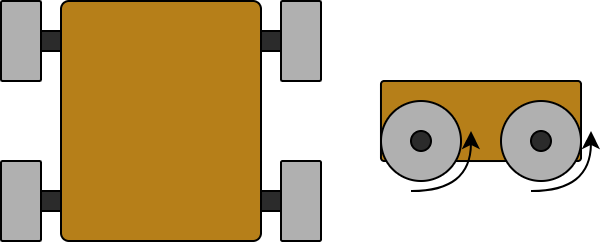
\includegraphics[width=3cm]{4_wheel_skid}} \\  
    \makecell[l]{2 Wheel \\ Differential \\ with Casters} &  \makecell[l]{Two driven wheels \\ with casters for free \\ rotation.} &  \makecell[l]{\\ 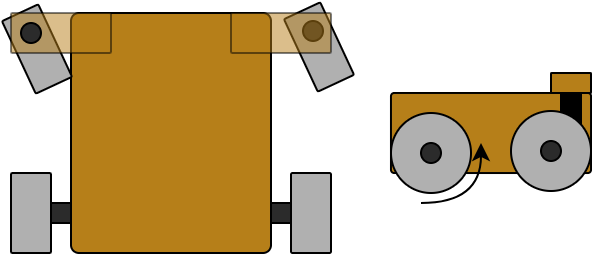
\includegraphics[width=3cm]{2_wheel_diff}} \\
    \makecell[l]{AWD \\ Standard \\ Steering} &  \makecell[l]{Four driven wheels \\ with standard \\differential steering.} &  \makecell[l]{\\ 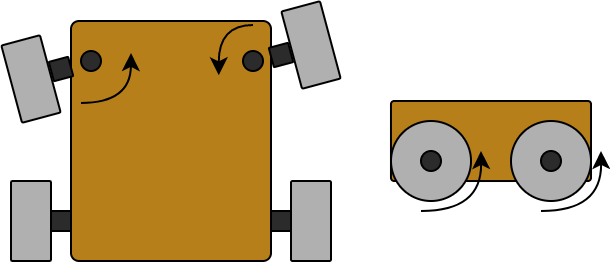
\includegraphics[width=3cm]{awd_standard_steer}} \\
    \makecell[l]{RWD \\ Standard \\ Steering} &  \makecell[l]{Two driven wheels \\ with standard\\ differential steering.} &  \makecell[l]{\\ 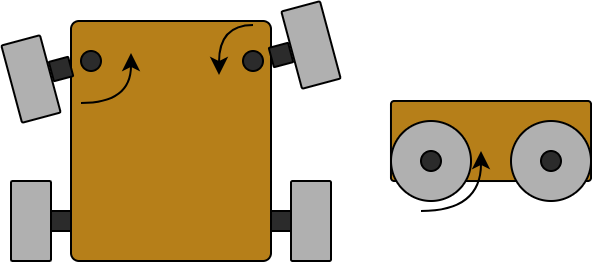
\includegraphics[width=3cm]{rwd_standard_steer}} \\
    \makecell[l]{Articulated} &  \makecell[l]{Four driven wheels \\ with center pivot \\ articulated steering.} &  \makecell[l]{\\ 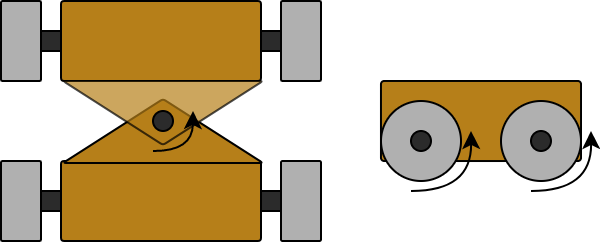
\includegraphics[width=3cm]{articulated}} \\
    \makecell[l]{Tracked} &  \makecell[l]{Two driven wheels \\ with tracks and \\ skid steering.} &  \makecell[l]{\\ 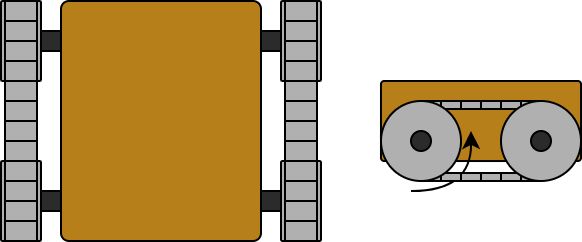
\includegraphics[width=4cm]{tracked}} \\
    \makecell[l]{3 Wheel \\ Delta} &  \makecell[l]{Three driven wheels \\ with immediate x, y, \\ and rotation control.} &  \makecell[l]{ 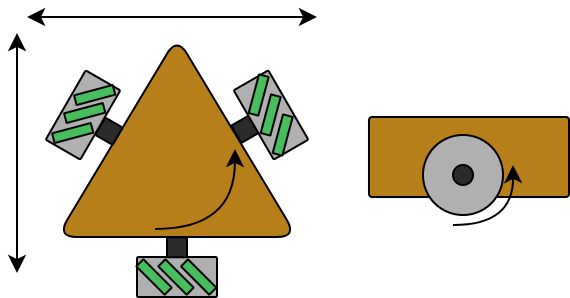
\includegraphics[width=3cm]{3_wheel_delta}} \\
    \makecell[l]{4 Wheel \\ Omniwheel} &  \makecell[l]{Four driven wheels \\ with immediate x, y, \\ and rotation control.} &  \makecell[l]{\\ 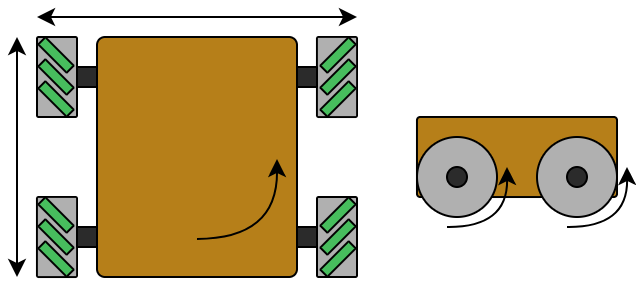
\includegraphics[width=3cm]{4_wheel_omniwheel}} \\
    
        \end{tabular}
    
    \end{adjustwidth}
    \end{table}





%%%%%%%%%%%%%%platform config table%%%%%%%%%%%%%%%%%%%%%%%% 
    \begin{table}[H]
    
    
    \caption{Platform Configuration Trade Study}
    \label{Tab:PlatformConfigTable}
    \begin{adjustwidth}{-1in}{-1in}
    \centering
    \setlength{\dashlinedash}{.5pt}
    \setlength\tabcolsep{4pt}
    \def\arraystretch{2}
    

    \begin{tabular}{lcccccccc}
    \hline 
    \\[-5ex]                                                                                      & \makecell{\\ \\ \sffamily\normalsize{Speed}} & \makecell{\\ \sffamily\normalsize{Wheel} \\ \sffamily\normalsize{Compaction}} & \makecell{\\ \\ \sffamily\normalsize{Stability}} & \makecell{\\ \sffamily\normalsize{Platform} \\ \sffamily\normalsize{Complexity}} & \makecell{\\ \sffamily\normalsize{Odometry} \\ \sffamily\normalsize{Accuracy}} & \makecell{\\ \sffamily\normalsize{Turning} \\ \sffamily\normalsize{Radius} } & \makecell{\sffamily\normalsize{Performance} \\ \sffamily\normalsize{on Uneven} \\ \sffamily\normalsize{Terrain}} & \makecell{\\ \\ \sffamily\normalsize{Score}} \\ 
    \makecell[l]{\sffamily Weights \\ (1-5)}                                            & 3     & 2                & 1         & 3                   & 4                 & 5                                          & 5                             &       \\ \hline
    
    \\[-3ex]
    \sffamily\makecell[l]{4 Wheel \\ Skid}                                             & 5     & 4                & 4         & 4                   & 1                 & 1                                          & 5                             & 73    \\ \hdashline 
    
    %jesus christ this row is a goddamn mess BUT YOU GOTTA DO WHAT YOU GOTTA DO
    \cellcolor{highlight}\sffamily\makecell[l]{2 Wheel \\ Differential \\ with Casters}& \multicolumn{1}{c}{\cellcolor{highlight}4} & \multicolumn{1}{c}{\cellcolor{highlight}3} & \multicolumn{1}{c}{\cellcolor{highlight}4} & \multicolumn{1}{c}{\cellcolor{highlight}5} & \multicolumn{1}{c}{\cellcolor{highlight}5} & \multicolumn{1}{c}{\cellcolor{highlight}5} & \multicolumn{1}{c}{\cellcolor{highlight}5} & \multicolumn{1}{c}{\cellcolor{highlight}107}   \\ \hdashline
    
    \sffamily\makecell[l]{AWD \\ Standard \\ Steering}                                 & 5     & 4                & 4         & 2                   & 4                 & 2                                          & 5                             & 84    \\ \hdashline
    \sffamily\makecell[l]{RWD \\ Standard \\ Steering}                                 & 5     & 4                & 4         & 3                   & 5                 & 2                                          & 5                             & 91    \\ \hdashline
    \sffamily\makecell[l]{ \\ Articulated \\ \quad }                                   & 3     & 4                & 2         & 1                   & 3                 & 2                                          & 5                             & 69    \\ \hdashline
    \sffamily\makecell[l]{\\ Tracked  \\ \quad}                                        & 2     & 5                & 5         & 3                   & 1                 & 5                                          & 5                             & 84    \\ \hdashline
   \sffamily\makecell[l]{3 Wheel \\ Delta}                                            & 1     & 3                & 1         & 1                   & 1                 & 5                                          & 1                             & 47    \\ \hdashline
    \sffamily\makecell[l]{4 Wheel \\ Omniwheel}                                        & 2     & 4                & 2         & 1                   & 5                 & 5                                          & 1                             & 69    \\ 
    \end{tabular}
  
    \end{adjustwidth}
    \end{table}
    
%%%%%%%%%%platform base table%%%%%%%%%%%%%%%%%%%%%%%%%%%%   
Once a base configuration was determined, a specific implementation of the platform needed to be chosen. Several off-the-shelf as well as DIY platforms were considered \cite{husqvarna} \cite{superdroid}. A DIY platform was chosen (Table \ref{Tab:PlatformBaseTable}).

    \begin{table}[H]
    \begin{adjustwidth}{-1.5in}{-1.5in}
    \centering
    \setlength{\dashlinedash}{.4pt}
    \setlength\tabcolsep{4pt}
    \def\arraystretch{1.8}
    \caption{Platform Base Trade Study}
    \label{Tab:PlatformBaseTable} 
    
    \vspace{1em}


    \begin{tabular}{lcccccccc}
    \hline
    \\[-5ex]
                                                               & \normalsize\sffamily\makecell{ {Ease} \\ { of }\\  {Integration}} &\normalsize\sffamily\makecell{ {Ease} \\  {of} \\  {Repair}} & \normalsize\sffamily\makecell{ {Ease} \\  {of} \\  {Construction}} & \normalsize\sffamily\makecell{ {Flexibility} \\  {for} \\  {Modifications}} & \normalsize\sffamily\makecell{\\ \\  {Cost}} & \normalsize\sffamily\makecell{ \\  {Lead-} \\  {time}} & \normalsize\sffamily\makecell{\\ \\  {Traction}} & \normalsize\sffamily\makecell{\\ \\  {Score}} \\
    \sffamily Weights (1-5)                                          & 3                   & 2              & 3                    & 5                              & 3    & 2        & 4        &       \\ \hline
    
    \\[-2ex]
    \multicolumn{1}{l}{\sffamily\cellcolor{highlight}Complete DIY}& \multicolumn{1}{c}{\cellcolor{highlight}4} & \multicolumn{1}{c}{\cellcolor{highlight}5} & \multicolumn{1}{c}{\cellcolor{highlight}2} & \multicolumn{1}{c}{\cellcolor{highlight}5} & \multicolumn{1}{c}{\cellcolor{highlight}4} & \multicolumn{1}{c}{\cellcolor{highlight}4} & \multicolumn{1}{c}{\cellcolor{highlight}5} & \multicolumn{1}{c}{\cellcolor{highlight}93}    \\ \hdashline
   \sffamily RC Lawnmower                                           & 5                   & 3              & 5                    & 4                              & 1    & 2        & 5        & 83    \\ \hdashline
    \sffamily\makecell[l]{Modify Robot \\ Lawnmower}                & 3                   & 3              & 4                    & 1                              & 1    & 4        & 2        & 51    \\ \hdashline
    \sffamily\makecell[l]{Modify Electric \\ Push Mower}             & 2                   & 2              & 3                    & 1                              & 2    & 5        & 1        & 44    \\ \hdashline
    \sffamily\makecell[l]{Modify Electric \\ Ride on Mower}         & 2                   & 1              & 3                    & 1                              & 3    & 5        & 5        & 61    \\ \hdashline
    \sffamily\makecell[l]{Stock Platform with \\ Mower Attached}    & 5                   & 3              & 5                    & 4                              & 1    & 3        & 3        & 77    \\ 
    \end{tabular}
    
    \end{adjustwidth}
    \end{table}
    
\subsection{Sensor Trade Study}

%%%%%%%%%%sensor capability table%%%%%%%%%%%%%%%%%%%%   
Once the platform was decided upon, analysis on different sensors and sensor combinations began. Sensors were evaluated individually first to establish baseline capability and relevance to the project. Then sensors were evaluated in different combinations, taking into account the results of the individual sensor study. The results showed that a stereo vision camera was the sensor that best fit the needs of GroundsBot (Table \ref{Tab:SensorCapabilitiesTable}).


    \begin{table}[H]
    \begin{adjustwidth}{-1.5in}{-1.5in}
    \setlength{\dashlinedash}{.4pt}
    \setlength\tabcolsep{4pt}
    \def\arraystretch{1.3}
    \centering


    \caption{Sensor Capabilities}
    \label{Tab:SensorCapabilitiesTable}
    
    \vspace{1em}

    \begin{tabular}{lcccccc}
    \hline
                                                                     & \normalsize\sffamily\makecell{ {Identify} \\  {Static}  \\  {Obstacles}} & \normalsize\sffamily\makecell{ {Identify} \\  {Dynamic} \\  {Obstacles}} & \normalsize\sffamily\makecell{ {Detect} \\  {Grass /} \\  {No Grass}} & \normalsize\sffamily\makecell{ {Functions} \\  {Outdoors} \\  {In Daylight}} & \normalsize\sffamily\makecell{ {Detect} \\  {Grass} \\  {Transitions}} & \normalsize\sffamily\makecell{ {Sense} \\ Driveable \\  {Land}} \\ 
        \hline
    \\[-2ex]
    \sffamily LiDAR                                                        & 5                         & 5                          & 0                       & 5                              & 0                        & 5                    \\ \hdashline
    \sffamily Camera                                                       & 3                         & 3                          & 5                       & 5                              & 5                        & 1                    \\ \hdashline
    
    \multicolumn{1}{l}{\sffamily\cellcolor{badhighlight!70}RGBD Camera }& \multicolumn{1}{c}{\cellcolor{badhighlight!70}5} & \multicolumn{1}{c}{\cellcolor{badhighlight!70}5 } & \multicolumn{1}{c}{\cellcolor{badhighlight!70}5 } & \multicolumn{1}{c}{\cellcolor{badhighlight!70}5 }   & \multicolumn{1}{c}{\cellcolor{badhighlight!70}0 } & \multicolumn{1}{c}{\cellcolor{badhighlight!70}5 } \\ \hdashline
    \sffamily\makecell[l]{Omnidirectional \\ Camera (upwards)}            & 3                         & 3                          & 0                       & 5                              & 0                        & 0                    \\ \hdashline
    \sffamily Stereo Camera                                                & 4                         & 3                          & 5                       & 5                              & 5                        & 3                    \\ \hdashline
    \sffamily Thermal Camera                                               & 1                         & 5                          & 0                       & 5                              & 0                        & 1                    \\ \hdashline
    \sffamily Sonar                                                        & 3                         & 3                          & 0                       & 5                              & 0                        & 2                   \\    
    \end{tabular}

    \end{adjustwidth}
    \end{table}
    
%%%%%%sensor trade study table%%%%%%%%%%%%%%%%%%%%%%%%%%%
    \begin{table}[H]
    \begin{adjustwidth}{0in}{0in}
    \setlength{\dashlinedash}{.4pt}
    \setlength\tabcolsep{4pt}
    \def\arraystretch{1.3}
    \centering
    
    \caption{Perception Sensor Trade Study}
    \label{Tab:PerceptionSensorTable}
    
    \vspace{1em}

    \begin{tabular}{lcccccc}
    \hline
    \\[-2ex]
                                                                     & \normalsize\sffamily\makecell{\\ \\  {Ability}} & \normalsize\sffamily\makecell{\\ \\  {Cost}} & \normalsize\sffamily\makecell{ {Hardware} \\  {Integration} \\  {Complexity}} & \normalsize\sffamily\makecell{ {Software} \\  {Integration} \\  {Complexity}} & \normalsize\sffamily\makecell{ \\  {Computational} \\  {Intensity}} & \normalsize\sffamily\makecell{\\ \\  {Score}} \\ 
    \sffamily Weights                                                      & 5       & 3    & 4                               & 5                               & 3                       &       \\ \hline
    \\[-2ex]
    \sffamily LiDAR + 1x Camera                                            & 4       & 2    & 3                               & 4                               & 3                       & 67    \\ \hdashline
    \sffamily LiDAR + Stereo Camera                                        & 5       & 1    & 3                               & 3                               & 2                       & 61    \\ \hdashline
    \sffamily\makecell[l]{Omnidirectional Camera + \\ Down Camera}        & 2       & 5    & 4                               & 2                               & 3                       & 60    \\ \hdashline
    \multicolumn{1}{l}{\sffamily\cellcolor{highlight}Stereo Camera Only}& \multicolumn{1}{c}{\cellcolor{highlight}3} & \multicolumn{1}{c}{\cellcolor{highlight}4} & \multicolumn{1}{c}{\cellcolor{highlight}5} & \multicolumn{1}{c}{\cellcolor{highlight}4} & \multicolumn{1}{c}{\cellcolor{highlight}4} & \multicolumn{1}{c}{\cellcolor{highlight}79}    \\ \hdashline
    \sffamily\makecell[l]{Thermal Camera + \\ LiDAR + Camera}             & 4.5     & 1    & 3                               & 2                               & 2                       & 53.5  \\ \hdashline
    \sffamily Many Cameras                                                 & 3       & 4    & 2                               & 2                               & 2                       & 51    \\ 
    
    \end{tabular}

    \end{adjustwidth}
    \end{table}


\newpage
\section{Cyberphysical Architecture}
\begin{figure}[H]
\centering
\def\svgwidth{\columnwidth}
\input{img/cyberphysical.pdf_tex}
\caption{Cyberphysical Architecture}
\label{fig:cyberphysical}
\end{figure}

  The user interface and IO subsystems are the contact points for the operator. The WiFi access point allows the user to load mowing boundaries from their laptop or mobile device. This also enables the user to download coverage reports and diagnostics. Status LEDs allow the operator to understand the system status at a glance, while safety beacons alert humans to GroundsBot's presence at a distance.\\

  GroundsBot uses its sensor suite to ensure a clean cut. GPS \cite{swiftnav}, IMU, and Motor Encoders are used for coarse localization while the cameras are used to ensure optimal grass overlap while cutting. Cameras and also enable GroundsBot to detect static and dynamic obstacles. A GPS RTK base station allows for tighter localization.\\

  GroundsBot's battery subsystem reports charge status to the CPU to prevent GroundsBot from becoming stranded. The battery subsystem also contains standard protection protocols including charge control, under-voltage lockout, and over-current protection. \\

  The CPU utilizes sensor information for localization, obstacle detection, and planning. After a local path is devised drive signals are sent to the motors. The CPU also logs coverage data and generates reports.\\

  The Drive Train contains motors and motor drivers to propel GroundsBot across a golf course. This also encompasses the mowing apparatus and mowing deck height control. \\

\newpage


\section{Current System Status}
  \subsection{Fall-semester targeted system requirements}
  todo
  Identify the system requirements and
  corresponding subsystems and system elements emphasized during the fall semester
  development. This goes first in this section in keeping with good systems engineering
  practice: identify your design requirements, then describe below the work you did to satisfy
  them.
  \subsection{Current system/subsystem descriptions/depictions}
   todo
   Describe and depict the subsystems developed during the spring semester. Start with an overall system depiction. Use design
  drawings, photographs, schematics, and other visual means to convey the status of your
  system/subsystems.
  \subsection{Modeling, analysis, and testing}
  todo
  Include a summary of any modeling, analysis, and testing
  you performed in order to design your system to specification and unit-test its components.
  \subsection{Performance evaluation against the Fall Validation Experiment (FVE)}
   todo
   Summarize how well your system performed against the scenario and metrics specified by your FVE.
  \subsection{Strong/weak points}
   todo
   Highlight current system strong and weak points and needed areas of
    refinement.

\section{Subsystem Descriptions}
  todo: delete this section?
  \subsection{UI}
  It is critical for the user to communicate a desired mowing path to the robot. This input method must be separate from the robot itself, allowing the user to be somewhere else as the robot mows autonomously. \\
  
  This will be achieved through a mobile device, either a dedicated tablet or the user's own smartphone. An app or website will be loaded onto this device and allow for the user to input a map outline that will be communicated to the robot. 
  
  \subsection{Hardware}
    \subsubsection{Platform}
      Based on the trade study, a differential drive system with two drive wheels and caster wheels will be used. Another trade study was used to narrow down the platform to a DIY platform instead of a preexisting platform. This custom platform will utilize aluminum extrusions, allowing for easy re-sizing of the platform as well as simple adjustment of the sensor mounts. Currently, motors and batteries from Discovery Robotics will be integrated, but alternate products may be also be considered. 
      
    \subsubsection{Mower}
      In addition to navigating a plot of grass, the system also needs to mow it. Given that a custom platform will be made, this will be done by attaching an existing electric push mower to the robot platform. Alternatively, it will also be possible to attach the blades from a manual reel mower to the platform. 
  
  \subsection{Software}
    \subsubsection{Planner}
      The planner subsystem consists of two parts: a global planner and a local planner. The global planner will take the user input from the UI and translate the input into a path that the robot will follow. This involves refining the outline that was provided by the user and then finding a path that will allow for maximum coverage of the selected area. \\ 
      
      The local planner will be responsible for adapting the route on-the-fly to avoid any obstacles that the robot may encounter. This system will also drive to and from the dock and cutting area. 
      
    \subsubsection{Localization and Perception}
      An accurate description of the robot global position and orientation will be obtained from this subsystem. This information may be obtained from a high-accuracy GPS system, such as RTK-GPS, but visual SLAM based methods will also be investigated. \\
      
      The vision system will also be used to detect boundaries of the grass as the robot approaches the boundary. For obstacle detection, our trade study determined that a stereo camera system would best fit the detection requirements. However, if needed, a LiDAR may be added to improve the detection accuracy. 
    
    \subsubsection{Mobility}
      The mobility subsystem will be responsible for controlling the robot motors. Part of this involves the robot going from point A to point B at any given time. Using current position information from the localization subsystem, this subsystem will find the next waypoint that will allow for the robot to follow the predetermined plan and then transmit the necessary motor control signals to move towards this waypoint. \\
      
      The cutter motor speeds will also be controlled by this subsystem. This subsystem must both detect the speed of the motor, as well as apply the correct motor signals to maintain a constant speed when the cutter encounters an obstacle. 

\newpage

\section{Project management}
\subsection{Work Breakdown Structure}
Present the three-level Work Breakdown Structure you
developed in the Systems Engineering class. Include whatever textual description is
necessary to make its contents clear.
\subsection{Schedule}
\subsubsection{Biweekly Spring Schedule}
Include a schedule with biweekly (every other week) granularity for the spring
semester.
\subsubsection{Milestone Evaluation}
Answer these key questions:
A. What are the major system development milestones in the remaining
schedule?
B. Are you behind, ahead of, or on schedule? If behind, how will you catch up?

\subsection{Test plan}
Present a high-level test plan for the spring semester including the spring validation experiment.
\subsubsection{Spring Milestones}
i. Use a table to identify capability milestones for these spring-semester Progress
Reviews (PR):
A. PR 7: Late January
B. PR 8: Mid-February
C. PR 9: Late February
D. PR 10: Mid-March
E. PR 11: Early April
F. PR 12: Mid-April
\subsubsection{Spring Validation Experiment}
ii. Describe the Spring Validation Experiment (SVE), to be conducted in late April-early
May, with greater detail than the other capability milestones, including these
essential elements:
A. The test conditions: location, needed equipment, size and nature of
operating area, etc.
B. A list of steps your system will be put through written in a sufficiently clear
way for someone with no knowledge of your project to be able to test the
robot.
C. A set of quantitative performance metrics that your system will be measured
against during the validation experiment. Typically, these metrics will be
written into the list of steps in the previous item.
D. Use graphics to the extent possible to illustrate your SVE.

\subsection{Budget}
i. Include a refined parts list.
ii. Answer these key questions:
A. What is your total budget?
B. What are the big-ticket items that comprise the majority of your budget?
C. How much/what percentage have you spent to date?
\subsection{Risk Management}
\subsubsection{Risks Update}
Provide an update on the risks you identified in the Preliminary Design Review (PDR)
and have been tracking/addressing since then.
\subsubsection{Risks}
As you did for the PDR, present the following (examples of which are given below),
updating both tables to reflect any changes since the PDR:
A. A Risk Management table with Risk ID, Risk, Requirement, Type, Likelihood,
Consequence, Mitigation.
B. A Risk Likelihood-Consequence Table

\section{Project Management}
\subsection{Work Plan}
\subsubsection{Tasks}
The GroundsBot work plan is shown in the list below. The plan is separated into high level categories and underlying subtasks. \\

\begin{itemize}
  \item [] \textbf{Chassis}
    \subitem Complete BOM
    \subitem Design Power Distribution and Sensor Integration PCBs % Changed to PCBs from PCBAs because we are "designing PCBs
    \subitem Design Chassis
    \subitem Design GPS RTK Base Station
    \subitem Acquire Parts
    \subitem Integrate Subsystems
  \item [] \textbf{Simulation}
    \subitem Design Simulation Environment
    \subitem Complete Cursory Simulations
  \item [] \textbf{Localization}
    \subitem Integrate GPS + RTK Localization
  \item [] \textbf{Perception}
    \subitem Develop Static Obstacle Detection
    \subitem Develop Dynamic Obstacle Detection
  \item [] \textbf{Planning}
    \subitem Develop Global Route Planner
    \subitem Develop Obstacle Rerouting
  \item [] \textbf{Control}
    \subitem Develop Motor Control
  \item [] \textbf{UI}
    \subitem Create Web Application for Mapping
\end{itemize}

   
\subsubsection{Schedule}
The full list of milestones is laid out below in Table \ref{Tab:table_milestones}\\ 

\begin{table}[H]
\def\arraystretch{1}

\caption{Project Milestones}
\label{Tab:table_milestones}


\begin{tabular}{ll}
\hline
\normalsize\sffamily{Deadline} & \normalsize\sffamily{Milestone}                            \\
\\
Progress Review 1 [OCT 17 2017] & Mechanical CAD Complete \\
    &Electrical CAD Complete                     \\
    &BOM Complete                                \\
    &Parts Ordered                               \\
    &ROS Environment Initialized                 \\
                                               \\
Progress Review 2 [OCT 26 2017] & Chassis Assembled with Mowing Apparatus     \\
    &ROS Simulation Environment Complete         \\
    &GPS RTK Base Station Complete               \\
                                              \\ 
Progress Review 3 [NOV 7 2017] 
    &GroundsBot System Integration Complete      \\
    &GPS RTK Integration Complete                \\
    &Control Systems Demo Complete               \\
                                              \\
Progress Review 4 [NOV 21 2017] 
  
    &GroundsBot Accepts GPS Waypoints            \\
    &GroundsBot Follows GPS Waypoints            \\
    &Teleoperation Test Complete                 \\
                                               \\
Fall Validation Experiment [NOV 28 2017] 
 
    &GroundsBot Follows Route From Web App       \\
    &GroundsBot Differentiates Grass From Other Objects \\
                                            \\
                                            
January 2018

    &Global Planning Algorithm Complete          \\
    &Static and Dynamic Obstacle Detection Complete\\
                                               \\
February 2018
  
    &Read User Map Input                        \\
    &GroundsBot Reroutes Around Obstacles       \\
                                              \\
March 2018 
  
    &Full Mapping UI Complete                   \\
    &GroundsBot Autonomously Cuts Lot           \\
                                              \\
April 2018 

    &Final System Tests Complete                \\                                            \\
\end{tabular}

\end{table}

\subsubsection{Progress Reviews}
\noindent
\textbf{Progress Review 1}: The goal for Progress Review 1 is to have all hardware design complete with parts on order. \\
 \textbf{Progress Review 2}: The goal for Progress Review 2 is to have an assembled frame/chassis, a full ROS simulation environment, and a completed GPS + RTK base station.\\

\subsection{System Validation Experiments}
\subsubsection{Fall Validation Experiment}

	The aim of the fall validation experiment is to test individual subsystems. As such many of the systems requirements set for GroundsBot will not be fully met. All tests to be performed have been designed to indicate significant progress towards reaching the system requirements. More specifically the team plans to test the base functionality of the mobility, localization, planning, and perception subsystems of GroundsBot. The details of the test are laid out below.
\\
\begin{center}
\textbf{Test 1:}
\end{center}
 \textbf{Location:} Field by Doherty Apartments \cite{interview-guenther}
\\
\textbf{Equipment:} GroundsBot, GroundsBot dock/RTK base station, laptop
\begin{enumerate}
  \item Power on GroundsBot next to its docking station
  \item Establish connection between GroundsBot and mobile device
  \item Input GPS waypoints following a typical zigzag pattern a groundskeeper might make when mowing a lawn
  \item Send waypoints to GroundsBot
  \item GroundsBot will navigate to each waypoint entered, in the order they were entered
  \item Once the last waypoint is reached, GroundsBot will navigate back to the docking station (Note: the docking station will not be one of the entered waypoints)
\end{enumerate}

\begin{center}
\textbf{Test 2:}
\end{center}
Test 2 has been designed to demonstrate base functionality of the perception subsystem. The team will present a perception algorithm capable of differentiating between grass (i.e. a mowable surface) and non-grass (i.e. a non-mowable surface.) This test will be performed outside of the fall validation experiment and a replay of the test will be displayed during the fall validation experiment.

\newpage
\subsubsection{Spring Validation Experiment}

	The spring validation experiment will be when the team will test the full GroundsBot system to demonstrate that all system requirements have been met. The details of the test are laid out below.
\begin{center}
 \textbf{Test 1: }
\end{center}
 \textbf{Location:} Field by Doherty Apartments \\
 \textbf{Equipment:} GroundsBot, GroundsBot dock/RTK base station, mobile device \\
\begin{enumerate}
  \item Power on GroundsBot next to its docking station
  \item Open UI on mobile interface and establish a connection with GroundsBot
  \item Have a new user (someone not on Team A) use the UI to draw an outline of the area to be mowed on a map including both static obstacles and a non-mowable surface (i.e. concrete)
  \item Use the UI to submit the mowing area to GroundsBot
  \item GroundsBot will develop a coverage plan of the area input by the user
  \item GroundsBot will navigate to the area to be mowed
  \item Once it has reached the edge of the mowing area it will begin mowing
  \item GroundsBot will detect and avoid any obstacles it comes across while mowing and will also only mow where there is grass
  \item Once GroundsBot has mowed the whole area it will return to the docking station
  \item GroundsBot will generate and transmit a coverage report to the UI indicating areas it could not mow
\end{enumerate}

\subsection{Team Member Responsibilities}
\begin{itemize}
  \item [] \textbf{Joe Phaneuf}
    \subitem  Team Lead
    \subitem  Systems Engineer
    \subitem  Project Management
  \item [] \textbf{Henry Chen}
    \subitem  Mechanical Design
    \subitem  Prototyping
    \subitem  Computer Vision
  \item [] \textbf{Josh Bennett}
    \subitem  Electrical Design
    \subitem  Mechanical Design
    \subitem  Instrumentation and Sensors
  \item [] \textbf{Adam Driscoll}
    \subitem  Control Systems
    \subitem  Perception
  \item [] \textbf{David Evans}
    \subitem  Power Distribution
    \subitem  Motion Planning
    \subitem  Localization and Mapping
\end{itemize}




\subsection{Provisional BOM}
A bill of materials is included in Table \ref{Tab:provisional_bom} with potential components and rough pricing information. Batteries and motors will be loaned to us from Discovery Robotics, reducing overall project cost. The batteries and motors shown in the BOM are backup components to be used if the loaned components do not fulfill project requirements.
\begin{table}[H]
\centering
\def\arraystretch{1.1}
\caption{Provisional BOM}
\label{Tab:provisional_bom}
\begin{tabular}{ llccl }
\hline
    \normalsize\sffamily {Manufacturer} & \normalsize\sffamily {Part No.} & \normalsize\sffamily {QTY} & \normalsize\sffamily {Cost} & \normalsize\sffamily {Description}\\
    \\[-.8ex]
    SuperDroid Robots & TD-111-135 & 1 & \$900 & Wheelchair Motors \& Encoders \\
	SuperDroid Robots & TE-240-030 & 1 & \$330 & Motor Controller \\
	SuperDroid Robots & TD-178-000 & 1 & \$150 & 13" Tiller Tires and Mounting \\
	Caster Connection & S-5210-PRB & 1 & \$70 & 10" Pneumatic Swivel Caster \\
	Smart Battery & SB2425 & 1 & \$700 & 24V 25aH Battery \\
    Smart Battery & DP-RS2 & 1 & \$165 & Battery Charger \\
    NVIDIA & Jetson TX2 Dev Kit & 1 & \$560 &  Embedded GPU \\
	ITEM & Extrusion & 1 & \$400 & Extrusions and Joints \\
	McMaster-Carr & Mechanical Components & 1 & \$500 & Misc Fasteners, Bearings \\
	DigiKey & Electrical Components & 1 & \$600 & Misc Connectors, Components \\[.5ex]
	\hline 
	\\[-2ex]
	Total: &&& \$4,375 &\\
	
    
\end{tabular}
\end{table}

\subsection{Risk Management}
\begin{table}[H]
\def\arraystretch{1.7}

\begin{tabular}{p{7cm}p{6cm}c}
 {Risk} &  {Management Strategy} &  {Risk Category}\\
\hline 
 \textbf{Too Few Features for Perception:} 
If we cannot consistently detect grass from non-grass features, perception subsystem will not be able to direct platform accurately
&
Install infrastructure such as fiducials to assist system in recognizing objects.
&
Technical\\

 \textbf{Team Falling Behind Due to Work:} 
Team may overestimate capability and overwhelm itself with assignments.
&
Prepare for risk by managing tasks and using buffer weeks. Mitigate effect by delaying milestones or cutting compromising targets.
&
Schedule\\
 \textbf{Localization Poor for Following Edges:} 
If our localization algorithms cannot accurately follow edge of lawn, system will not mow lawn effectively.
&
Prepare by understanding criticality of localization. Mitigate effect by changing scope of mowing problem or adding infrastructure to assist.
&
Technical\\
 \textbf{Injury from Spinning Blade:} 

Our system has a dangerous cutting instrument. It can injure a team member or a bystander.
&
Prepare by making sure team understands the risk of spinning blade. Put warning lights and sounds to alert bystanders when testing.
&
Technical\\

 \textbf{Poor Weather for Validation Experiments:} 
Poor weather on demonstration days would prevent us from system from performing.
&
Team monitors upcoming weather before validation experiments.  Records the validation experiment before hand and replays in the case of inclement weather conditions.
&
Schedule\\

 \textbf{Team Member Has Family Constraints:} 
Any team member could experience a family emergency or responsibility that occupies their time and focus. One specific concern is Josh's wife is pregnant and expecting in December.
&
Mitigate the effect on entire team by spreading work across several team members and communicating consistently with absent team member to keep them in the loop.
&
Personal\\

 \textbf{Platform Devastating Event:} 
Platform could have electrical, thermal, or kinetic event that leads to its destruction.
&
Team designs platform with risk in mind, and manages parts reserve to quickly rebuild platform if necessary.
&
Technical\\

 \textbf{Subsystem Harder Than Expected:} 
Any subsystem could require more work than expected, taking away focus from other subsystems.
&
Team can prepare by focusing on critical subsystems first, and may revise scope related to subsystem if necessary.
&
Technical\\

\textbf{Not Enough Capital for Development:} 
There is a risk our system requires more money than initially allocated.
&
To mitigate the effect of this event, team will maintain strong relationship with sponsor by providing consistent communication of development progress. Team may also reach out to other sponsors or donors.
&
Schedule\\
\end{tabular}
\end{table}

\section{Conslusions}
\subsection{Lessons Learned}
Key lessons learned during the fall semester.
\subsection{Spring Key Activities}
Resultant key activities during the spring semester.

\begingroup
\newpage
\section{References}
\renewcommand{\section}[2]{}% %Suppress bibliography header, doesn't work with toc
\begin{thebibliography}{}
\bibitem{clubbenchmarking} 
http://www.clubbenchmarking.com/blog/golf-course-maintenance-how-much-should-you-spend
\bibitem{husky} 
https://www.clearpathrobotics.com/husky-unmanned-ground-vehicle-robot/
\bibitem{husqvarna} 
http://www.husqvarna.com/us/products/robotic-lawn-mowers/
\bibitem{swiftnav} 
https://www.swiftnav.com/store?category=GNSS+Modules
\bibitem{superdroid} 
https://www.superdroidrobots.com/shop/item.aspx/prebuilt-2wd-66in-lawn-mower-wc-sold/1983/
\bibitem{interview-duxbury} 
Duxbury, Jeff [Bob O’Connor Golf Course Superintendent]. (2017, September 16). Personal interview.
\bibitem{interview-guenther} 
Guenther, Steve [Carnegie Mellon University Director of Facilities Operations]. (2017, September 22). Personal interview.
\end{thebibliography}
\endgroup

\end{document}

